\chapter{Evaluation of the Developed Local Path Planner} \label{cha:Eval}

\section{Introduction}
This section will evaluate the performances of the clothoidal LPT (the main focus of \cref{cha:Design} and contribution of this thesis) by comparing it with its predecessor, the circular LPT (discussed in \cref{sec:ColFreeTraj,sec:LPTreview}). First, the planning performance of both LPTs is assessed in \cref{sec:EvalPPP}. Two different path planning scenarios will be presented, requiring the planner to plan a trajectory through a narrow opening. One of the concerns raised in the conclusion of the design of the clothoidal LPT is the calculation time needed to calculate a path set that contains more paths compared to the circular path set. Time performances of both LPTs will therefore be analyzed in \cref{sec:EvalTP} in order to calculate the extra time needed to evaluate the additional paths from the clothoidal LPT. Some concluding remarks on the evaluation of the developed clothoidal LPT are given in \cref{sec:EvalConc}.

In order to objectively compare both LPTs, the curvature constraints on the path discussed in \cref{sec:WheelchairPlatform} are applied to the circular LPT. The procedure reviewed in \cref{sec:LPTreview} is performed, starting from 500 discrete input velocity pairs ($v,\omega$) but paths yielding a curvature $\kappa > \kappa_{max}$ are discarded. This results in a circular LPT composed of 250 trajectories (both forward and backward), shown in \cref{fig:MPCircVWPair_Eval}. The clothoidal LPT used for this evaluation is the same as shown in \cref{fig:LSLClothoid} and is composed of 1500 trajectories (forward and backward). Turning on the spot rotations were also discarded during this evaluation. 

\begin{figure}[!htbp]
	\centering
	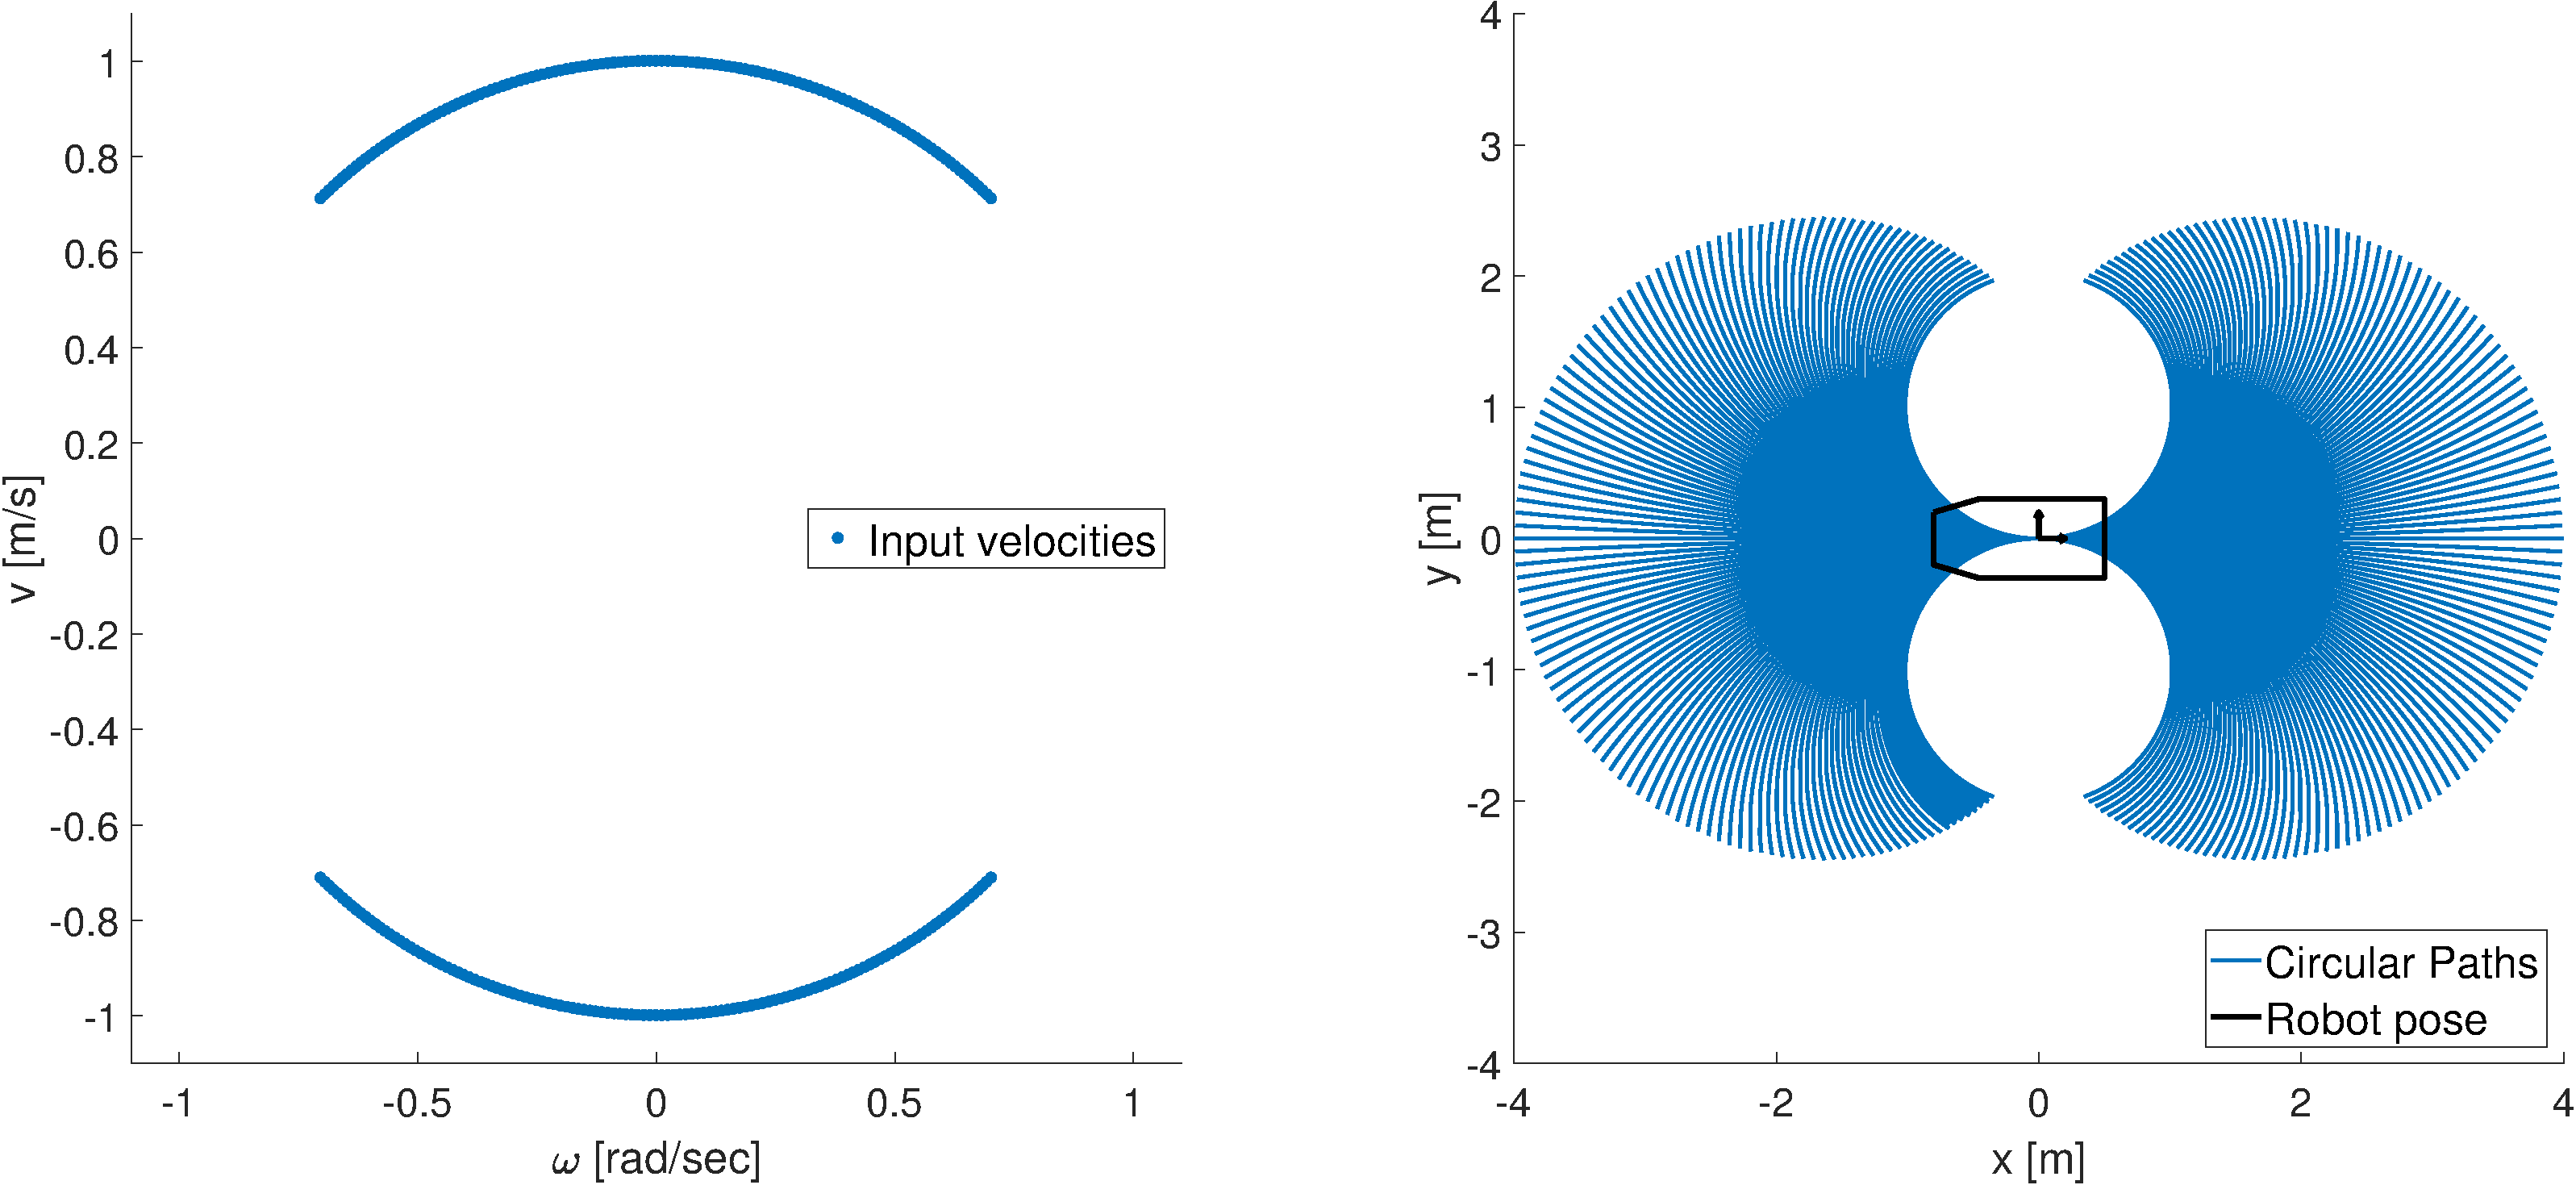
\includegraphics[width=\textwidth]{MPCircVWPair_Eval.pdf}
	\doublecaption{Input velocities (left) integrated over a period of  $\Delta t = 4 s$ to obtain 250 circular paths complying with the kinematic constraints (right)}{(adapted from \cite{DemeesterEtAl2012}).
	\label{fig:MPCircVWPair_Eval}}
\end{figure}

\newpage

\section{Path Planning Performances} \label{sec:EvalPPP}
This section evaluates the path planning performance of the circular and clothoidal LPTs. The first benchmark consists of driving forward through a doorway (\cref{sec:EvalForwardDoor}); for the second benchmark, the wheelchair has to drive backwards into an elevator (\cref{sec:EvalBackElev}). Both benchmarks are inspired by real-world environments. The first consists of driving in the robot laboratory of the Department of Mechanical Engineering of the KU Leuven whilst the second involves entering the elevator in the corridor leading to this same laboratory.

\subsection{Forward Driving Through a Doorway} \label{sec:EvalForwardDoor}
In this situation, the sAMR has to drive through a doorway to enter the robot laboratory. First, a single successful situation is shown for both LPTs. Then, a thorough analysis between the circular and clothoidal LPT is provided, by trying to plan a path through the doorway by starting from different start poses in the corridor leading to the laboratory. An overview of the different planning performance outcomes along with a histogram are provided to evaluate both LPTs.

\subsubsection{Visual Inspection}
\Cref{fig:EnterRobotLab_Footprint} shows a successful, collision-free path going through the doorway using both LPTs. One can visually inspect the collision-free nature of each path by plotting the geometry of the wheelchair along the path and checking whether this collides with an obstacle. The green path indicates the path which is simulated to be the closest to the user's intention.

\begin{figure}[!htbp]
	\centering
    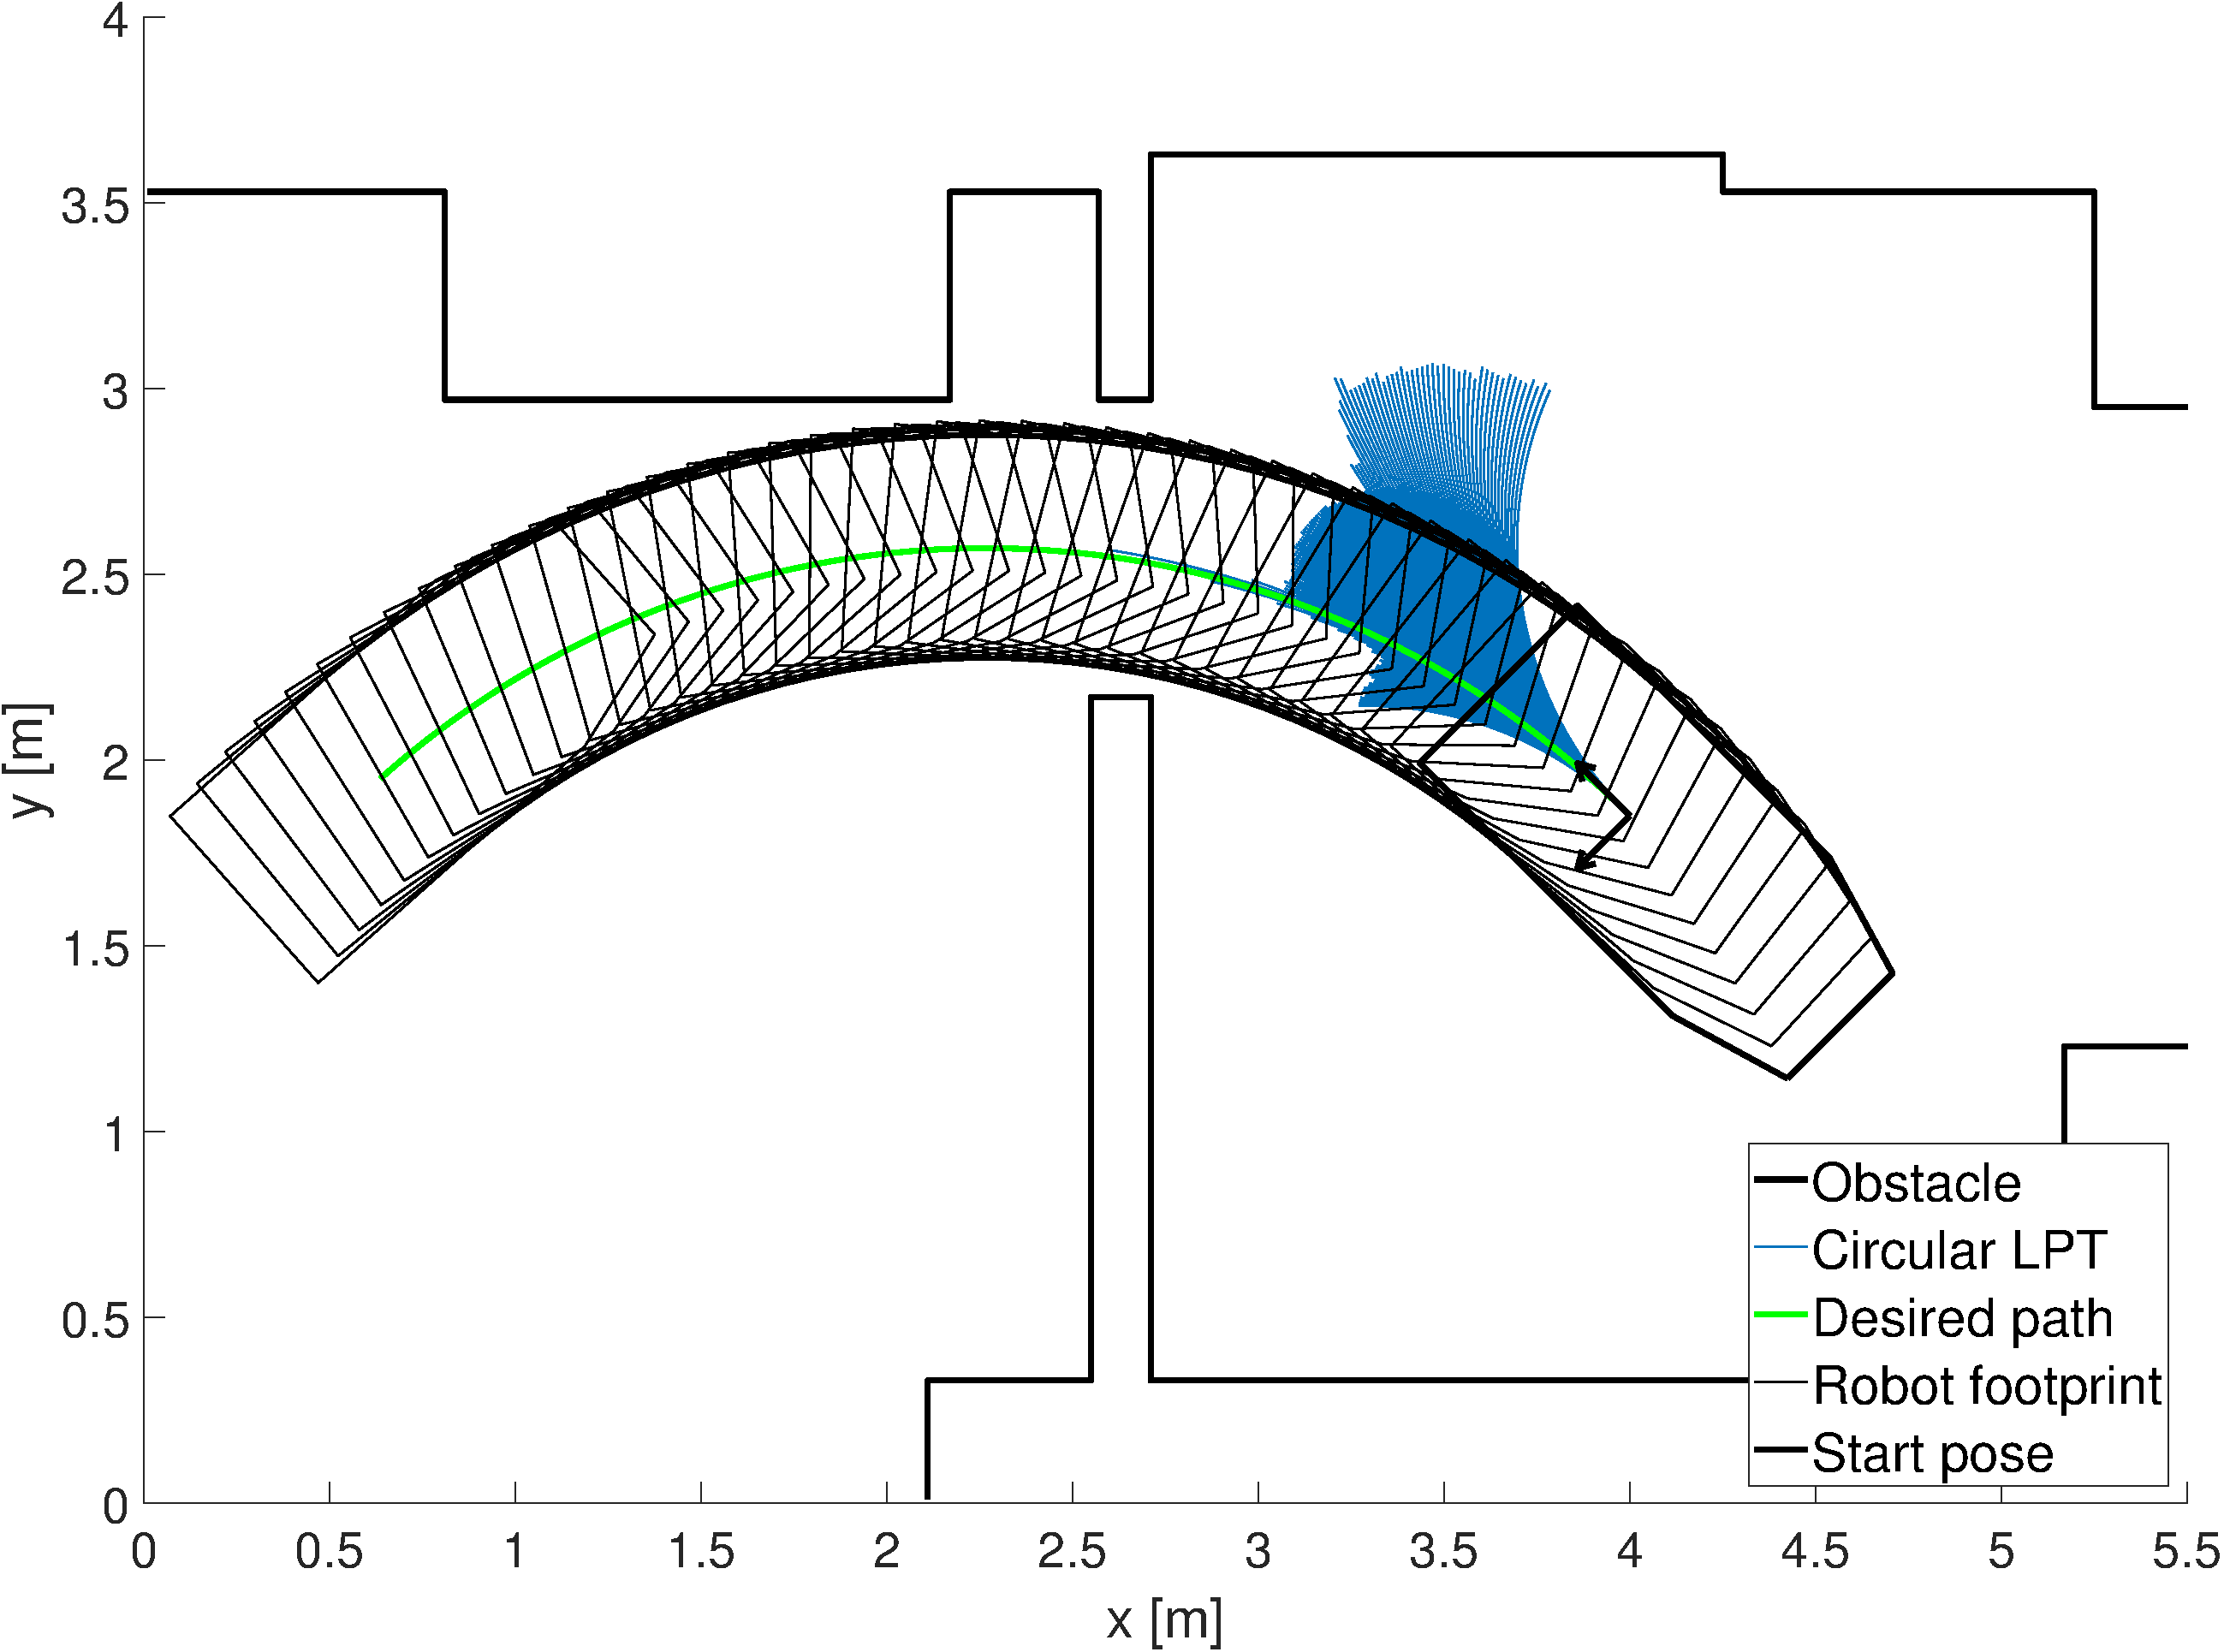
\includegraphics[width=0.45\textwidth]{EnterRobotLabCirc_Footprint.pdf}
    \hfill
    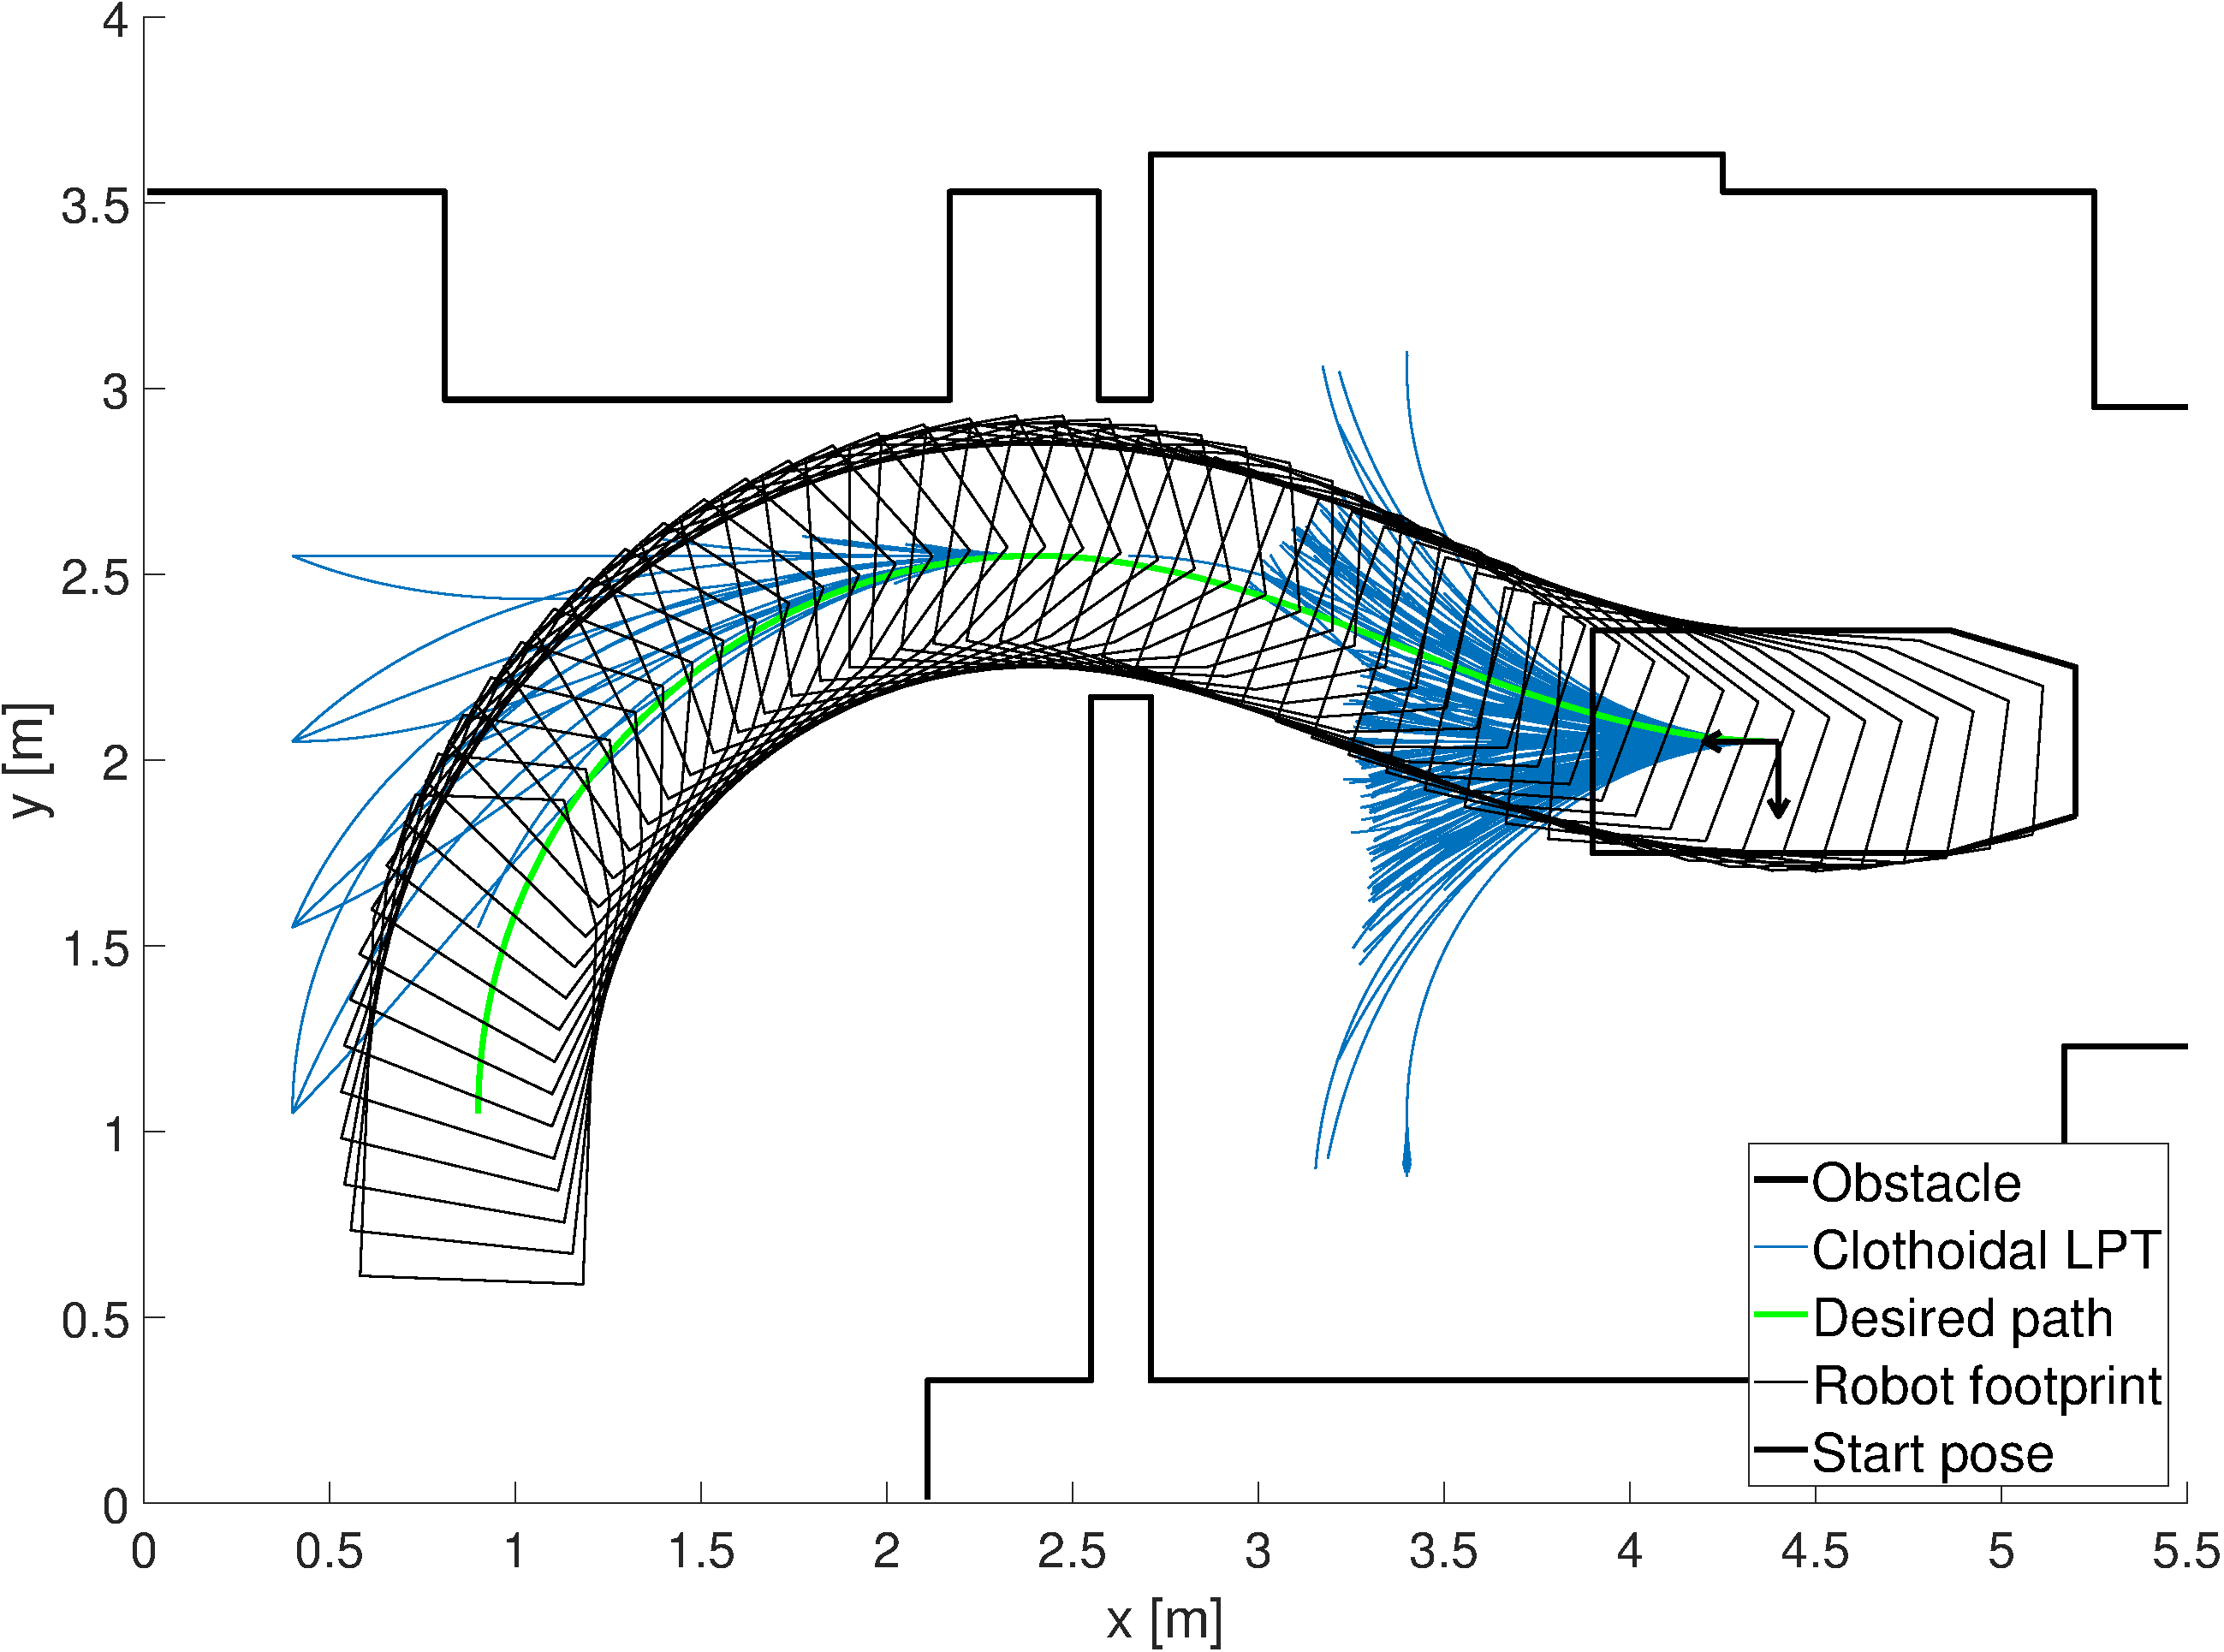
\includegraphics[width=0.45\textwidth]{EnterRobotLabCloth_Footprint.pdf}
     \doublecaption{Visual inspection of the selected path going through the doorway of the robot laboratory}{by plotting the footprint of the wheelchair along the selected path. (left) A successful path based on the circular LPT. (right) A successful path based on the clothoidal LPT. The footprint of the robot does not overlap with the environment, yielding collision-free paths for both LPTs.\label{fig:EnterRobotLab_Footprint}}
\end{figure}

\newpage

\subsubsection{Comparison Between the Circular and Clothoidal LPT}
%TODO not clear target and region
% Let's discuss this this evening
A uniform set of start poses are generated to assess the planning performances of both LPTs.
This is shown in \cref{fig:BenchmarkSetup} by performing the following steps:
\vspace{1em}
\begin{enumerate}
\item The test region (red polygon) defines uniformly spaced start positions (dots) with distance $dx$.
\item At each start position, a uniformly distributed set of start orientations, defined by $\theta_{range}$ and $\theta_{res}$ are aligned  with the target position (green star), creating a set of start poses. Then, each start orientation is rounded to the nearest multiple of $\theta_{res}$.
\item Poses resulting in a collision with the environment are removed.
\item If a path of the LPT originating from a start pose reaches the goal region (green polygon), that pose is defined as successful. The number of paths going through the goal region is not taken into account (e.g. \Cref{fig:EnterRobotLab_Footprint} shows a successful start pose for each LPT).
\item Successful start poses are divided in three cases:
\begin{enumerate}
	\item Only the circular LPT achieved to plan a path reaching the goal area
	\item Both LPTs achieved to plan a path reaching the goal area. 
	\item Only the clothoidal LPT achieved to plan a path reaching the goal area.
\end{enumerate}
\end{enumerate}

\begin{figure}[!htbp]
	\centering
	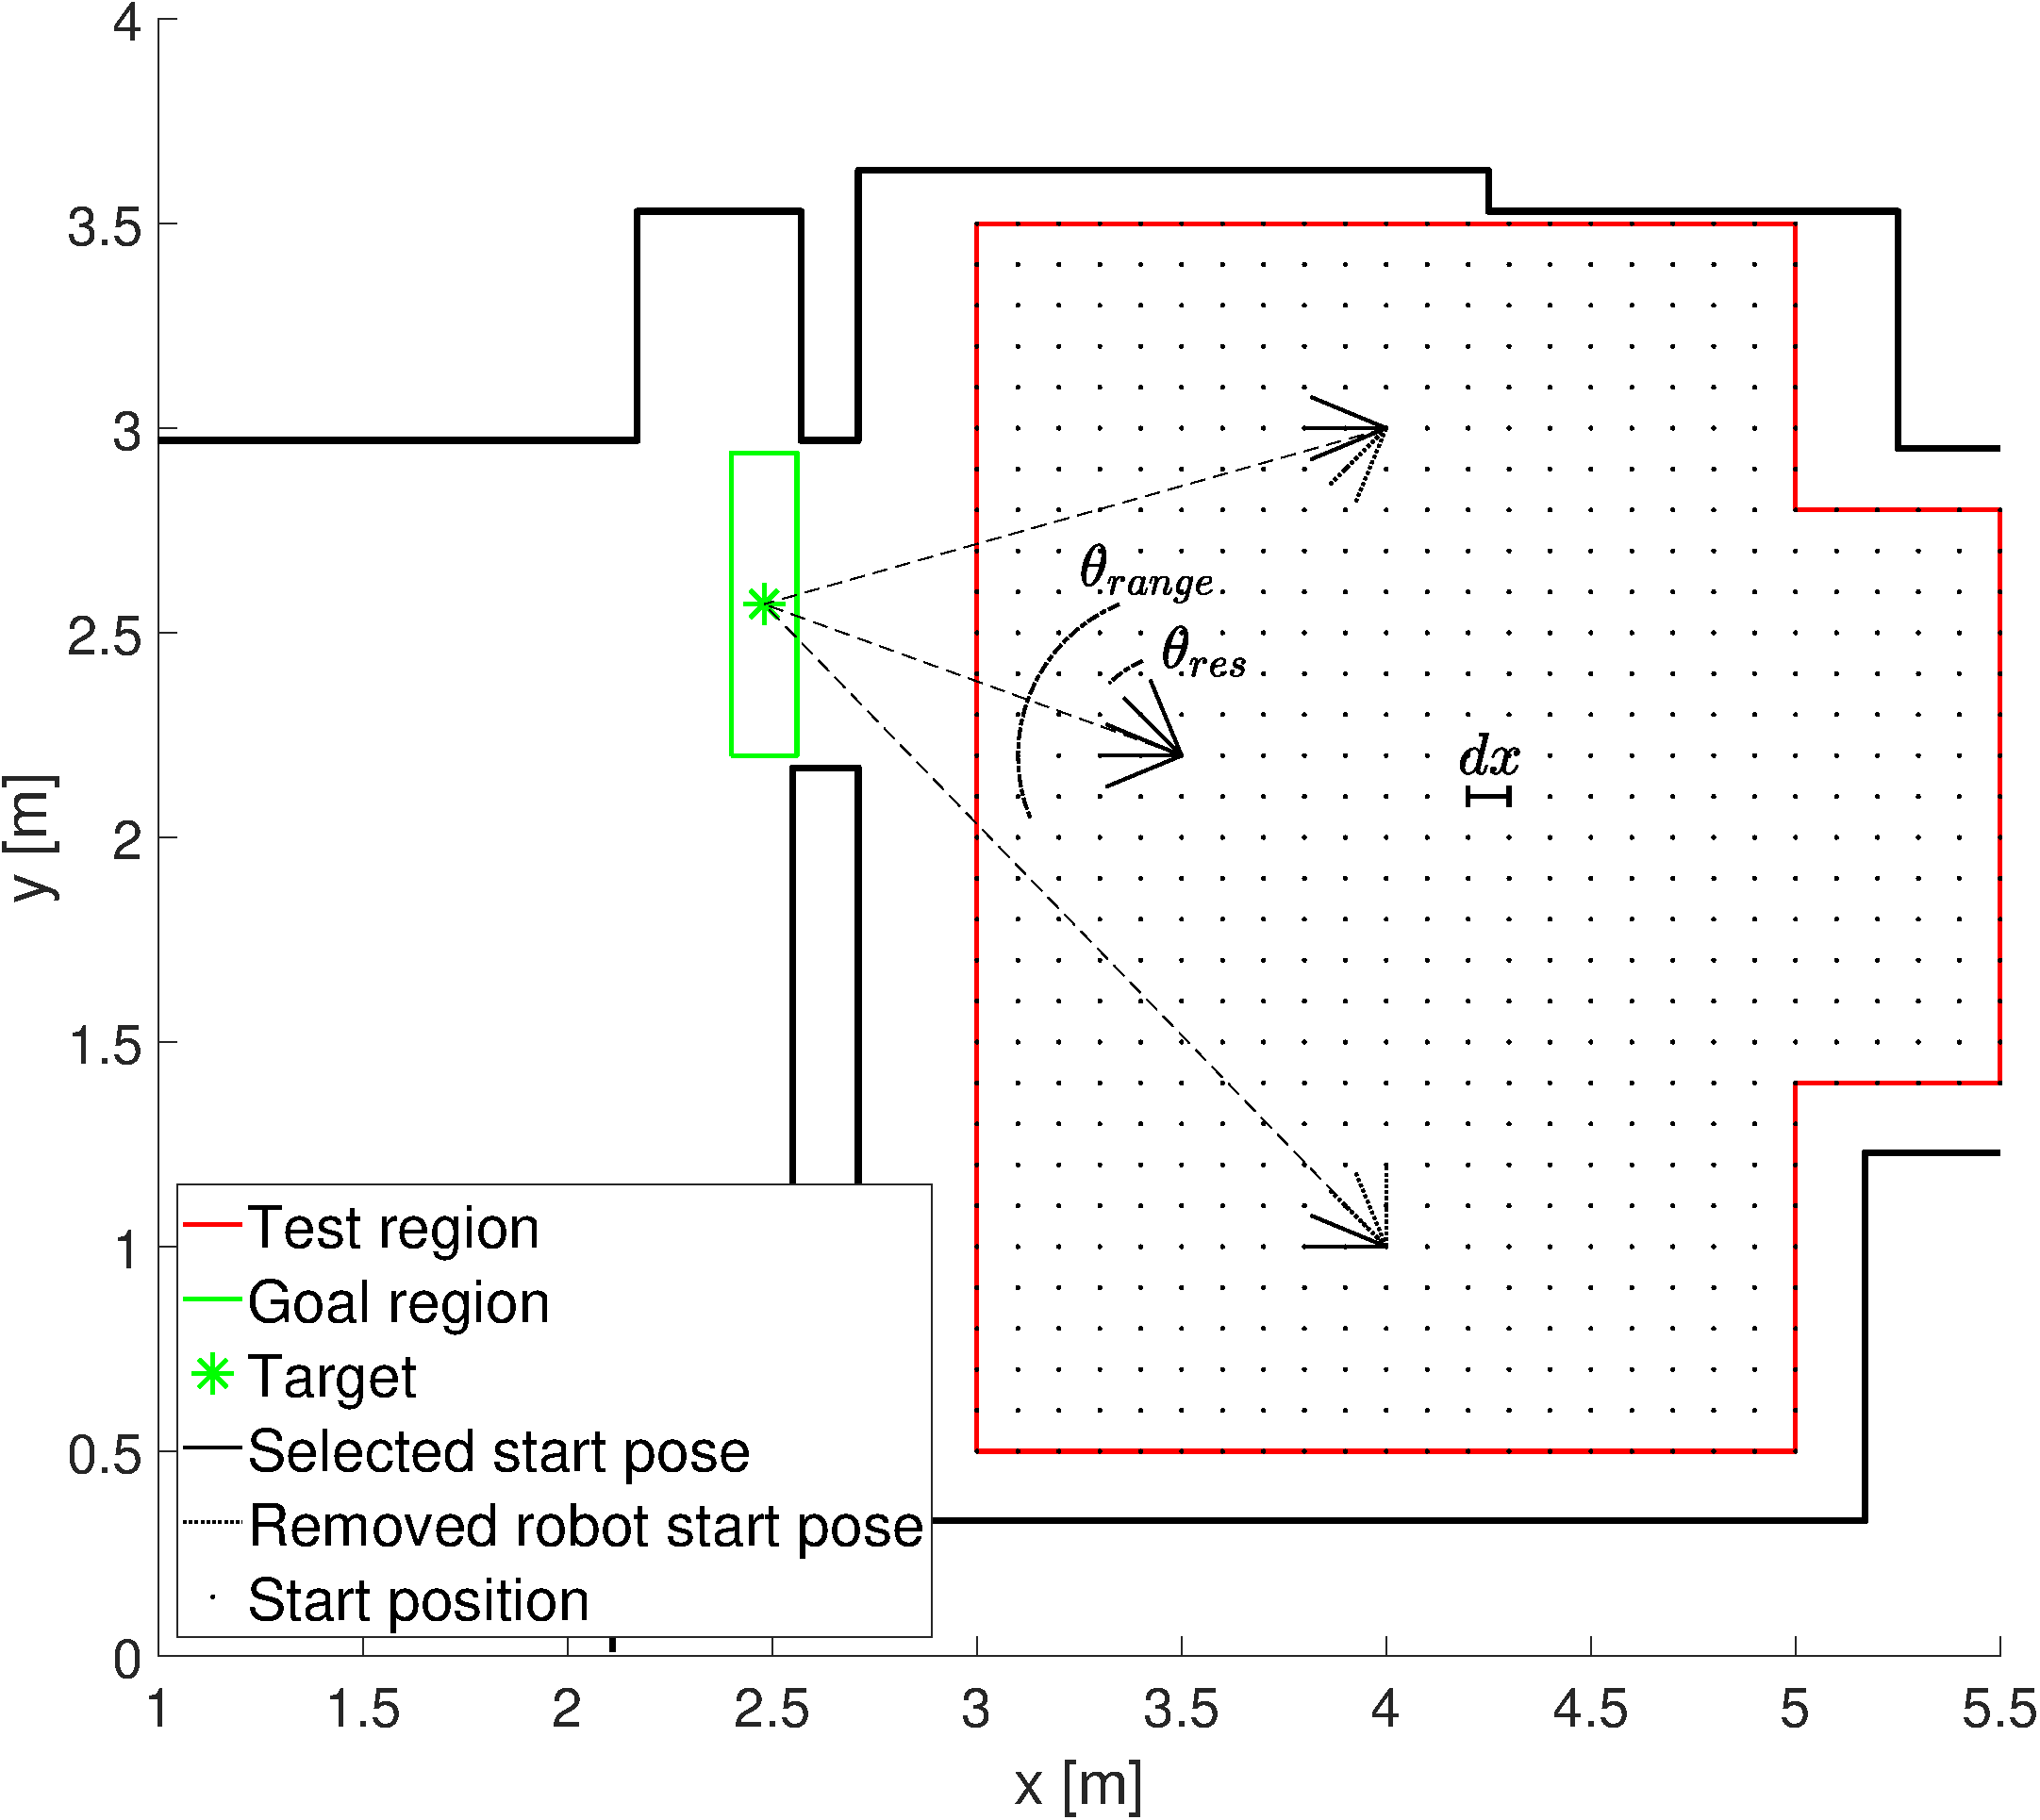
\includegraphics[width=.8\textwidth]{BenchmarkSetup.pdf}
    \doublecaption{Setup parameters of the uniformly distributed set of start poses.}{Start positions are uniformly spread with a distance of $dx=10cm$ between each other. The discrete set of start orientations are defined by $\theta_{range}= 90\degree$ and $\theta_{res}=\frac{90}{32}\degree$ and are aligned with the goal target. The last operation consists of rounding the start orientations to the nearest multiple of $\theta_{res}$ value to ensure a better uniformity.\label{fig:BenchmarkSetup}}
\end{figure}

\vspace{1em}

The final outcome when following this procedure is shown in \cref{fig:EnterRobotLabEval_result} along with a histogram of the occurrence of the three different cases in \cref{fig:EnterRobotLabEval_hist}. The unique successful start poses based on circular, common and clothoidal LPTs are shown respectively in red, black and green. The width of the doorway from the corridor to the robot laboratory is 80 cm while the width of the wheelchair is 60cm.

\newpage

From this outcome, several important conclusions can be drawn:
\begin{itemize}
\item Since straight paths are common to both LPTs, poses in front of the goal region obtain the same result for the circular and clothoidal LPT.
\item The majority of the paths from start poses at the lower end of the figure are achieved by the circular LPT. This is because those paths only require a circular arc to enter the doorway. Since the circular LPT is composed of a uniformly spread set of circular trajectories, this LPT is favored, compared to the clothoidal LPT.
\item From the moment the required trajectory is more complex (for example, \cref{fig:EnterRobotLab_Footprint} (right) the clothoidal LPT is the only LPT able to plan a path.
\item As per the histogram provided in \cref{fig:EnterRobotLabEval_hist}, the majority (87\%) of the poses with a successful path are generated by the clothoidal LPT, which demonstrates that for this first benchmark, the lack of uniformly spread circular trajectories is not so crucial, as only 13\% of the total amount of successful start poses are uniquely found by using the circular LPT.
\end{itemize}

\begin{figure}[!htbp]
	\centering
    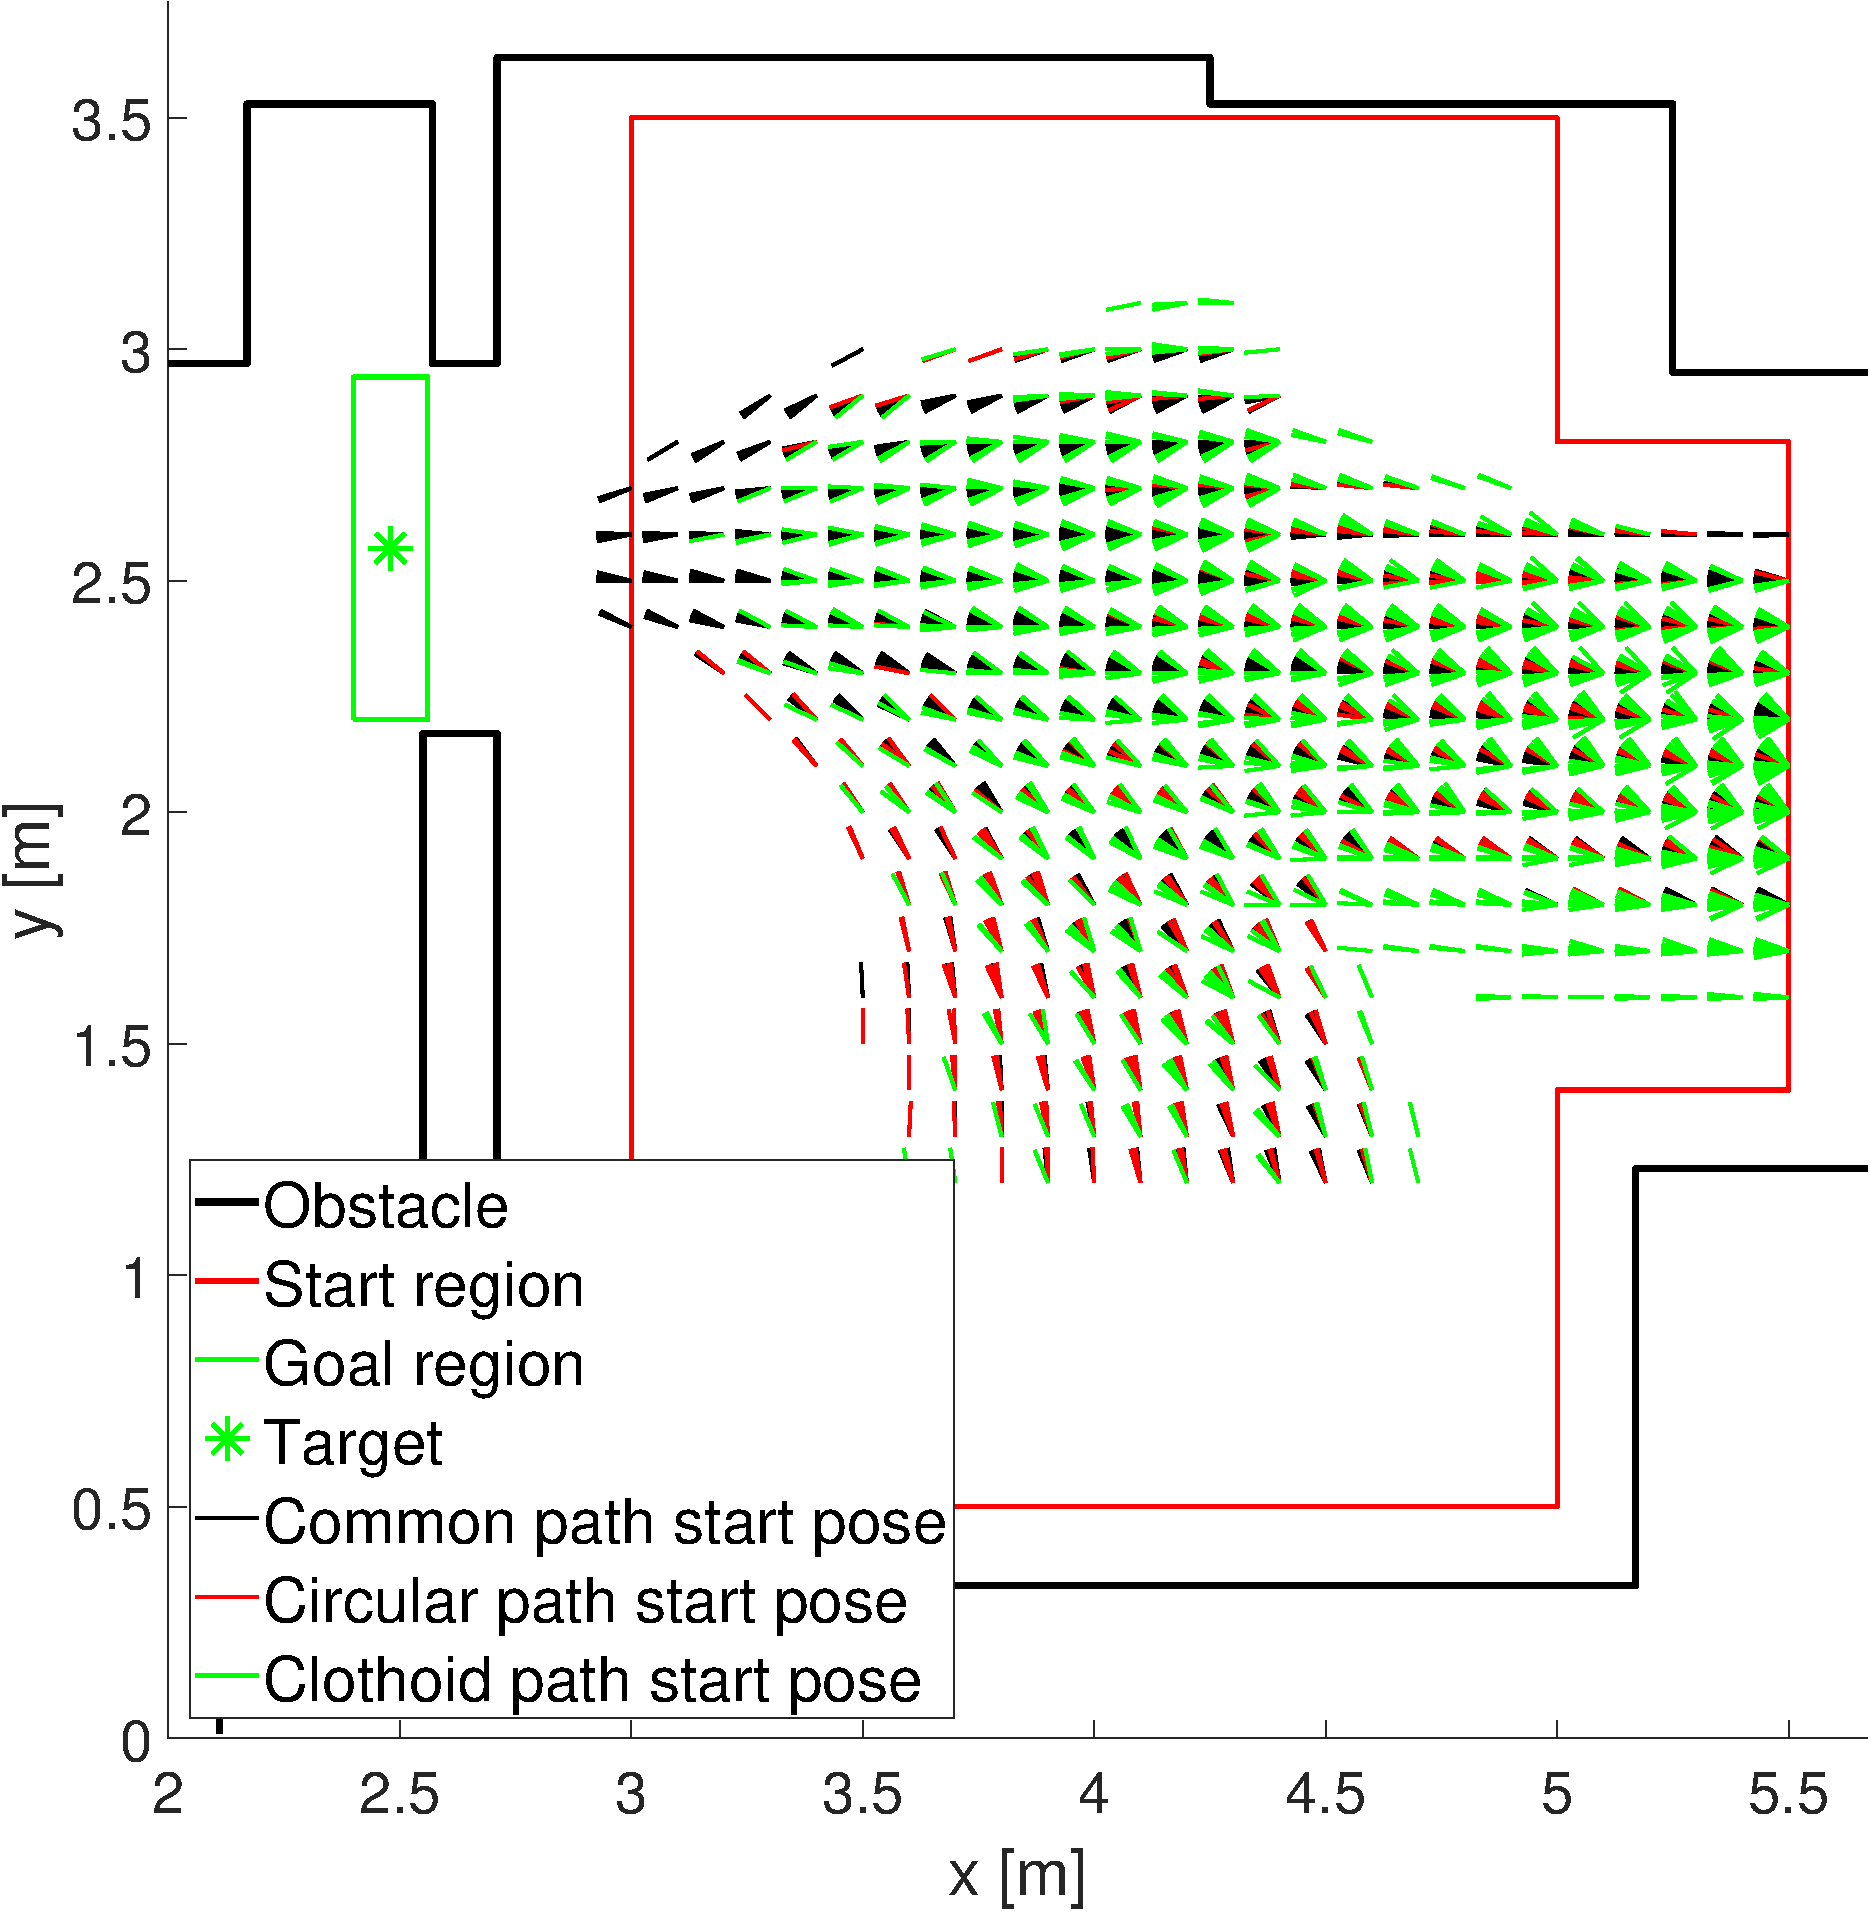
\includegraphics[width=0.85\textwidth]{EnterRobotLabEval_result.pdf}
     \doublecaption{Successful start poses for each LPT finding a path through the doorway of the robot laboratory}{separated in the three different cases.\label{fig:EnterRobotLabEval_result}}
\end{figure}

\begin{figure}[!htbp]
	\centering
    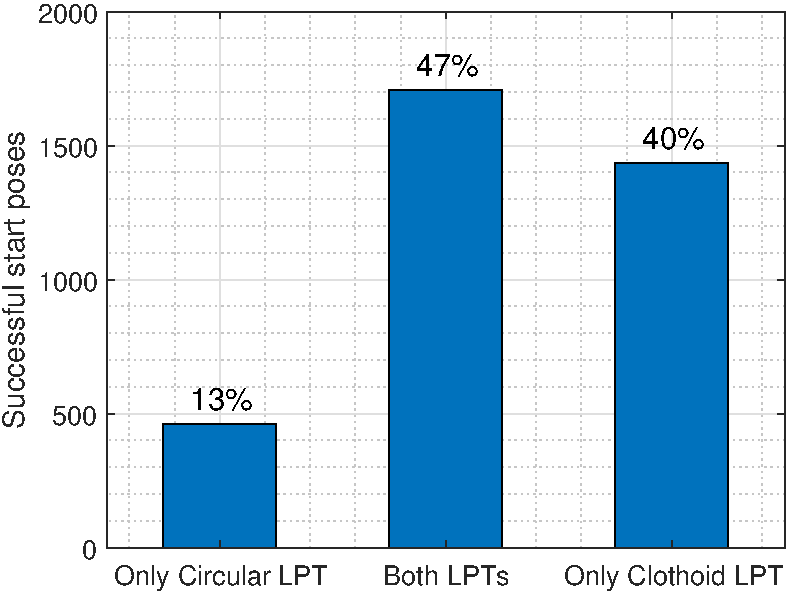
\includegraphics[width=0.5\textwidth]{EnterRobotLabEval_hist.pdf}
     \doublecaption{Histogram showing the outcome of the different cases of driving through the doorway of the robot laboratory.}{There are in total 3604 successful start poses, from which 1708 are common to both LPTs. Whereas 460 are only from the circular LPT and 1436 from the clothoidal LPT. \label{fig:EnterRobotLabEval_hist}}
\end{figure}

\newpage

\subsection{Backwards Driving in an Elevator} \label{sec:EvalBackElev}
In this situation, the sAMR must drive in reverse from a corridor into an elevator. First, a single successful situation is shown for both LPTs. Then, an in-depth comparison between the circular and clothoidal LPTs will be given of their attempts to reach the elevator by starting from different start poses in the corridor leading to the elevator. An overview of the different planning performances along with a histogram will be provided to evaluate both LPTs. This benchmark is inspired by the situation described in \cite{VanderPoortenEtAl2012}, where the circular LPT is unable to plan a trajectory leading to the elevator when the wheelchair is located in the corridor. The width of the elevator is 90 cm while the width of the wheelchair is 60cm.

\subsubsection{Visual Inspection}
\Cref{fig:EnterLift_Footprint} shows a successful, collision-free path going in reverse through the doorway of the elevator whilst using both LPTs. One can visually inspect the collision-free nature of each path by plotting the geometry of the wheelchair along the path and checking whether this collides with an obstacle. The green path indicates the path simulated to be the closed to the user’s intention.

\begin{figure}[!htbp]
	\centering
    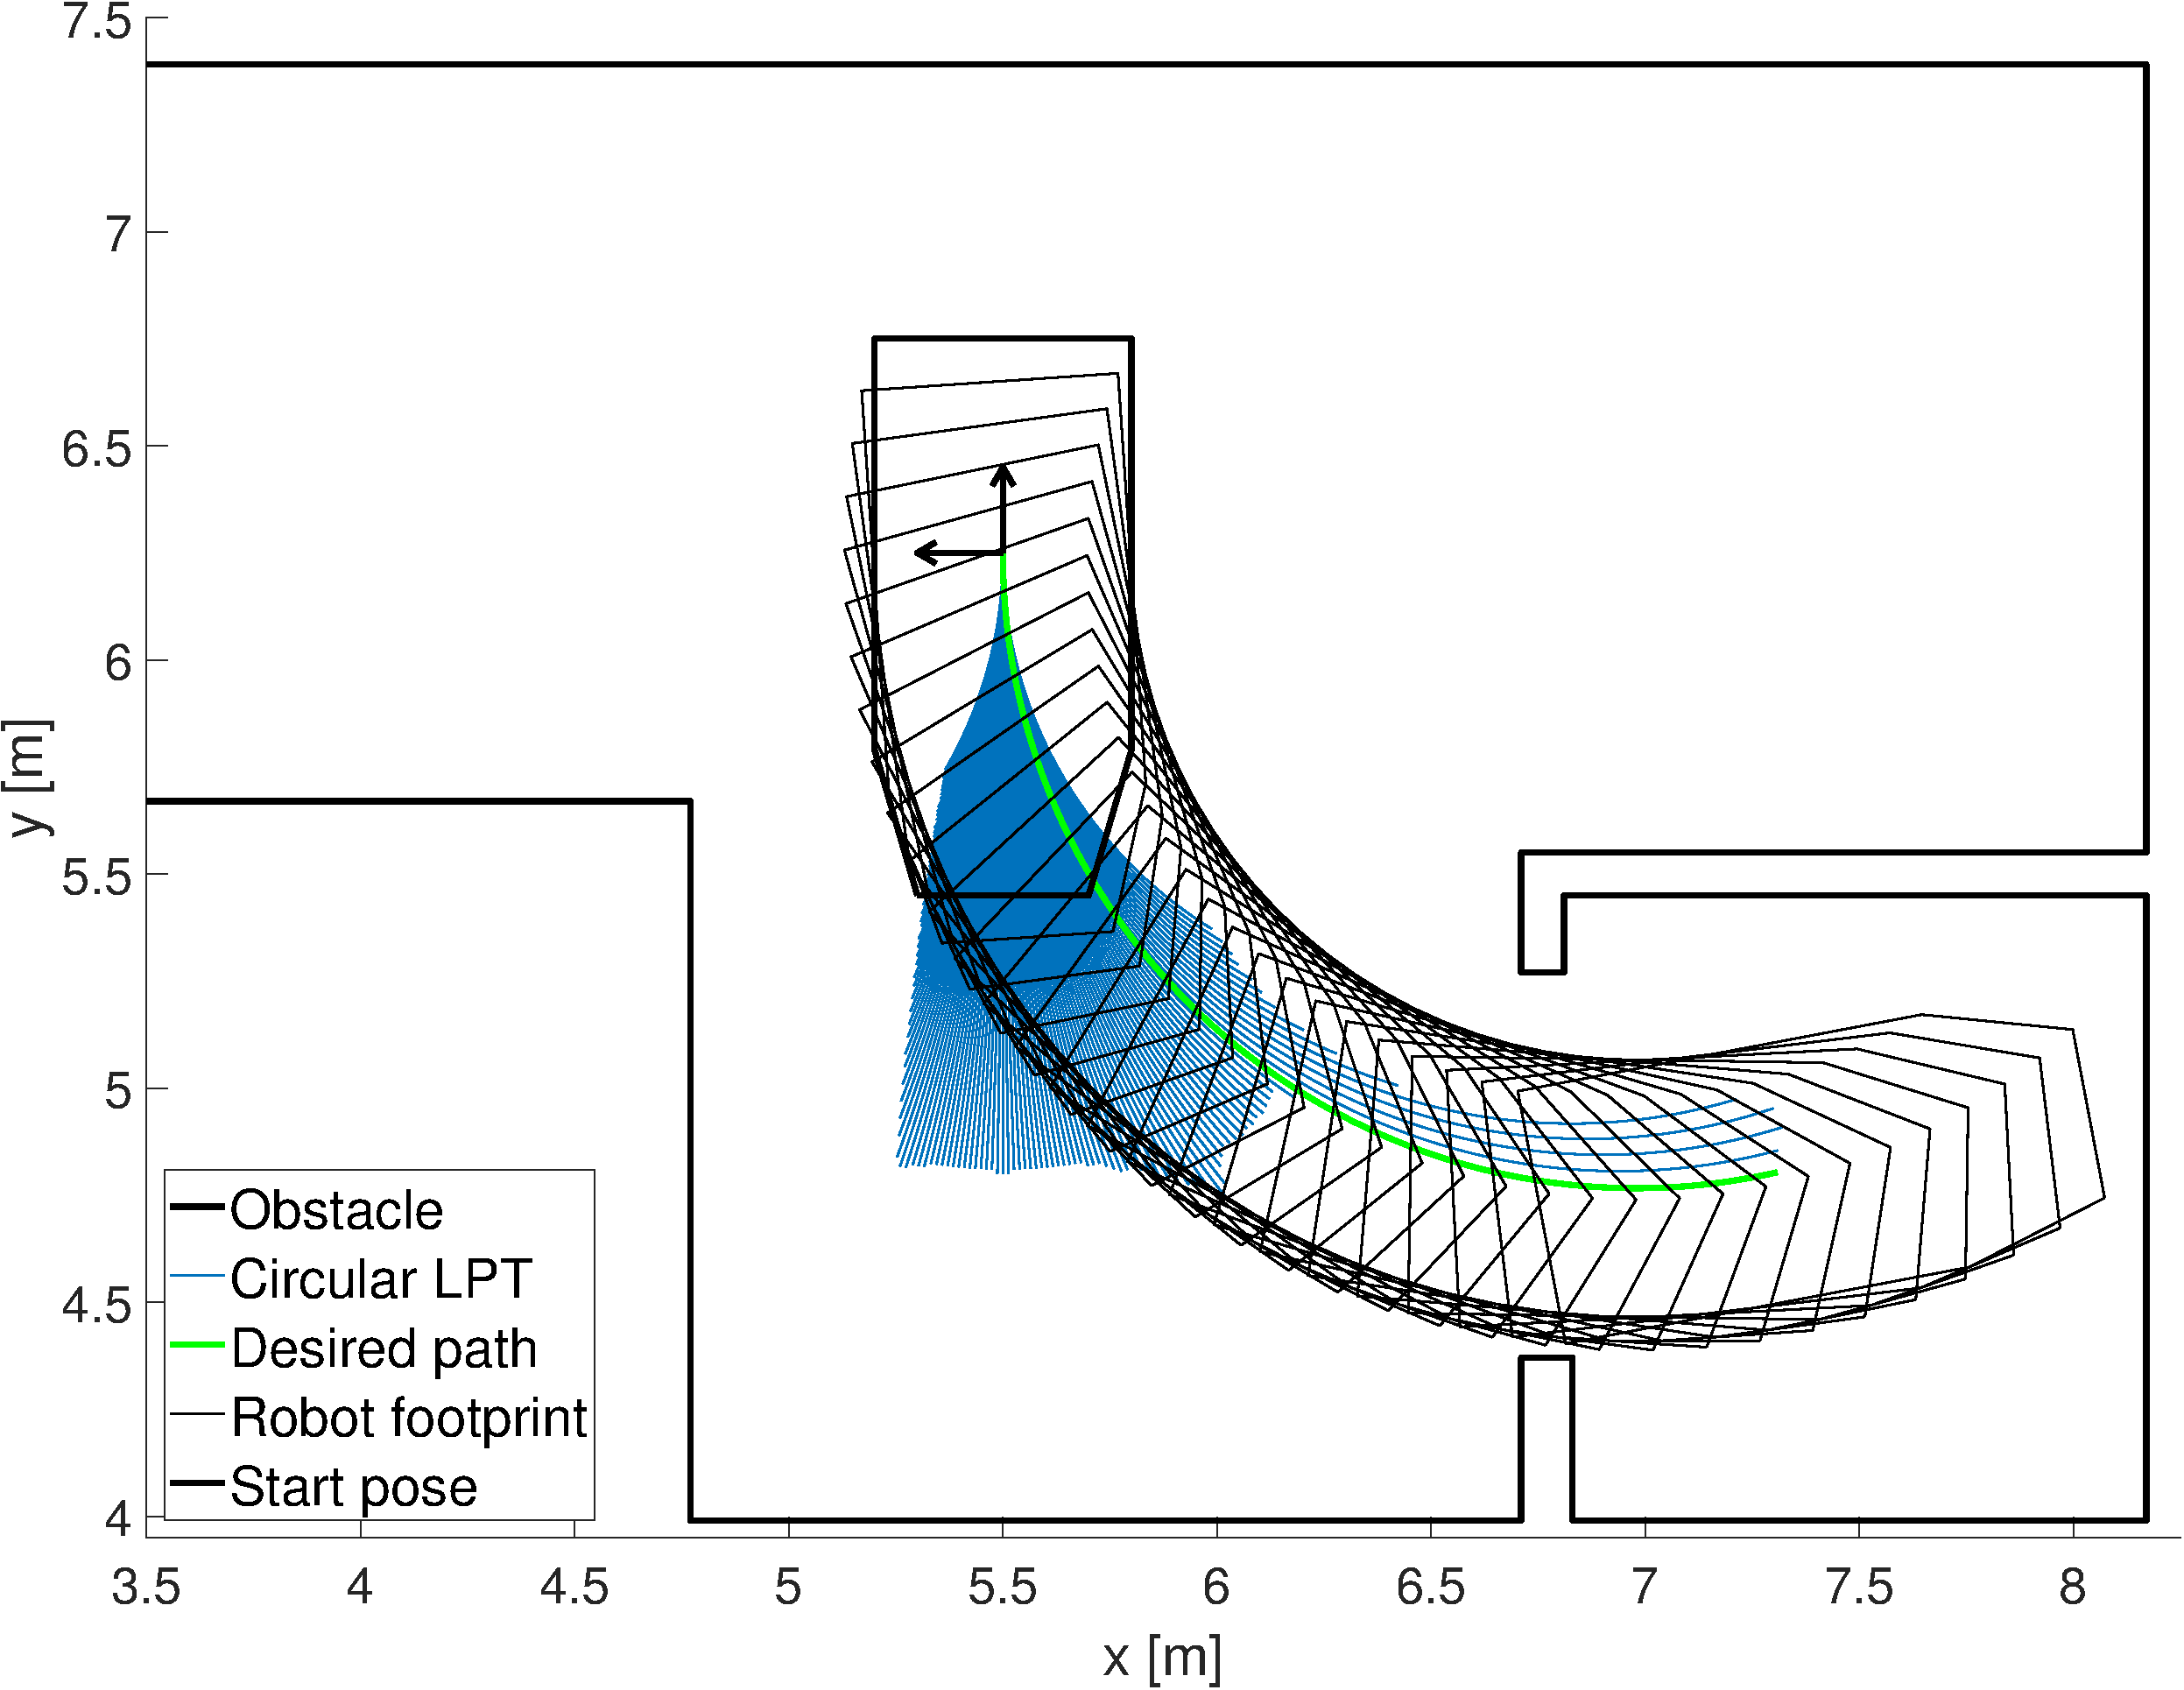
\includegraphics[width=0.45\textwidth]{EnterLiftCirc_Footprint.pdf}
    \hfill
	 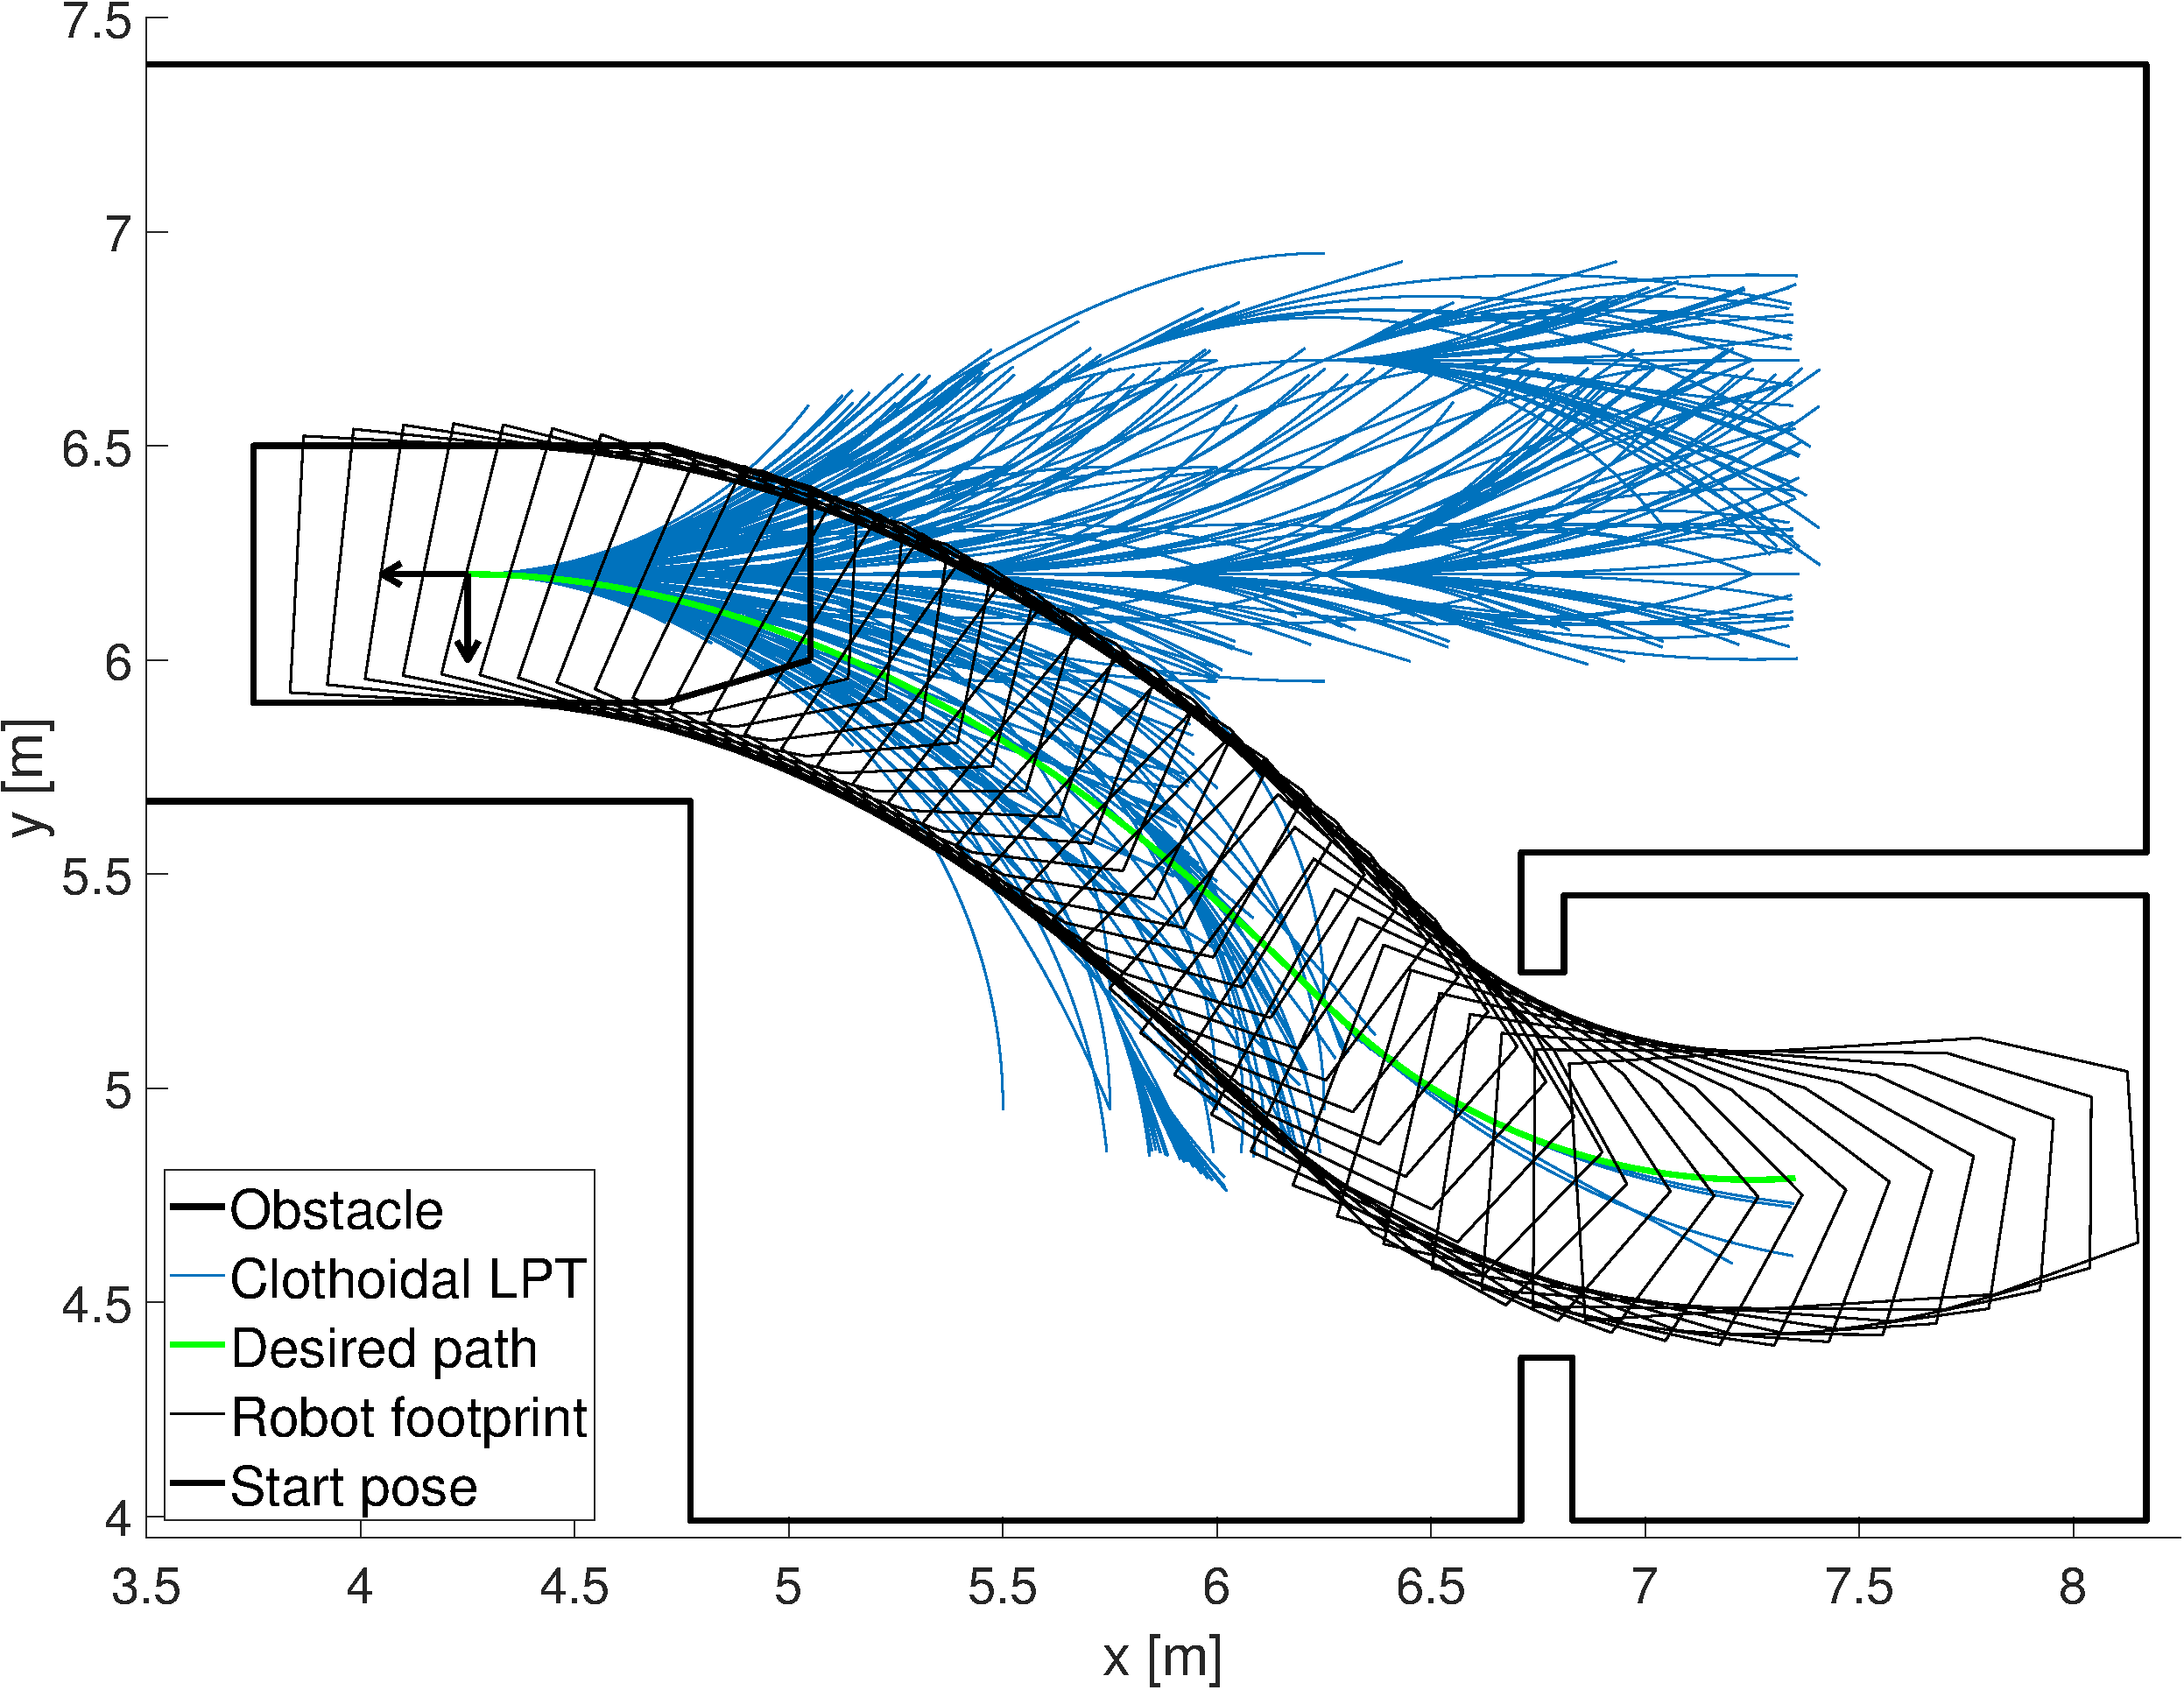
\includegraphics[width=0.45\textwidth]{EnterLiftCloth_Footprint.pdf}
     \doublecaption{Visual inspection of the selected path going in reverse through the doorway of the elevator}{by plotting the footprint of the wheelchair over the selected path. (left) A successful path based on the circular LPT. (right) A successful path based on the clothoidal LPT. The footprint of the robot does not overlap with the environment, proving that both cases yield a collision-free path.\label{fig:EnterLift_Footprint}}
\end{figure}

\newpage

\subsubsection{Comparison Between the Circular and Clothoidal LPT}
The same procedure as provided in \cref{fig:BenchmarkSetup} is applied for this benchmark.  From this outcome, several important conclusions can be drawn:
\begin{itemize}
\item The majority of the common start poses are found at the right of the start region, before the beginning of the corridor. 
\item From the moment the start pose of the wheelchair is located further away in the corridor, only the clothodial LPT manages to find a trajectory to the elevator.
\item This outcome confirms the comment in \cite{VanderPoortenEtAl2012}, that from the moment a trajectory leading to a certain destination becomes too complex, the circular LPT is unable to find a path. Recall from \cref{sec:PlanRec} that the collision-free trajectories also model the user’s intention. Since no paths can be found in the corridor leading to the elevator, there will be only limited guidance for the wheelchair user. By contrast, the clothoidal LPT performs very well in the corridor and is able to plan a path to the elevator from far in corridor.
\item The above outcomes are confirmed by the histogram shown in \cref{fig:EnterLiftEva_hist}. Nearly all the start poses are successful when using the clothoidal LPT (98\%).
\end{itemize}

\begin{figure}[!htbp]
	\centering
    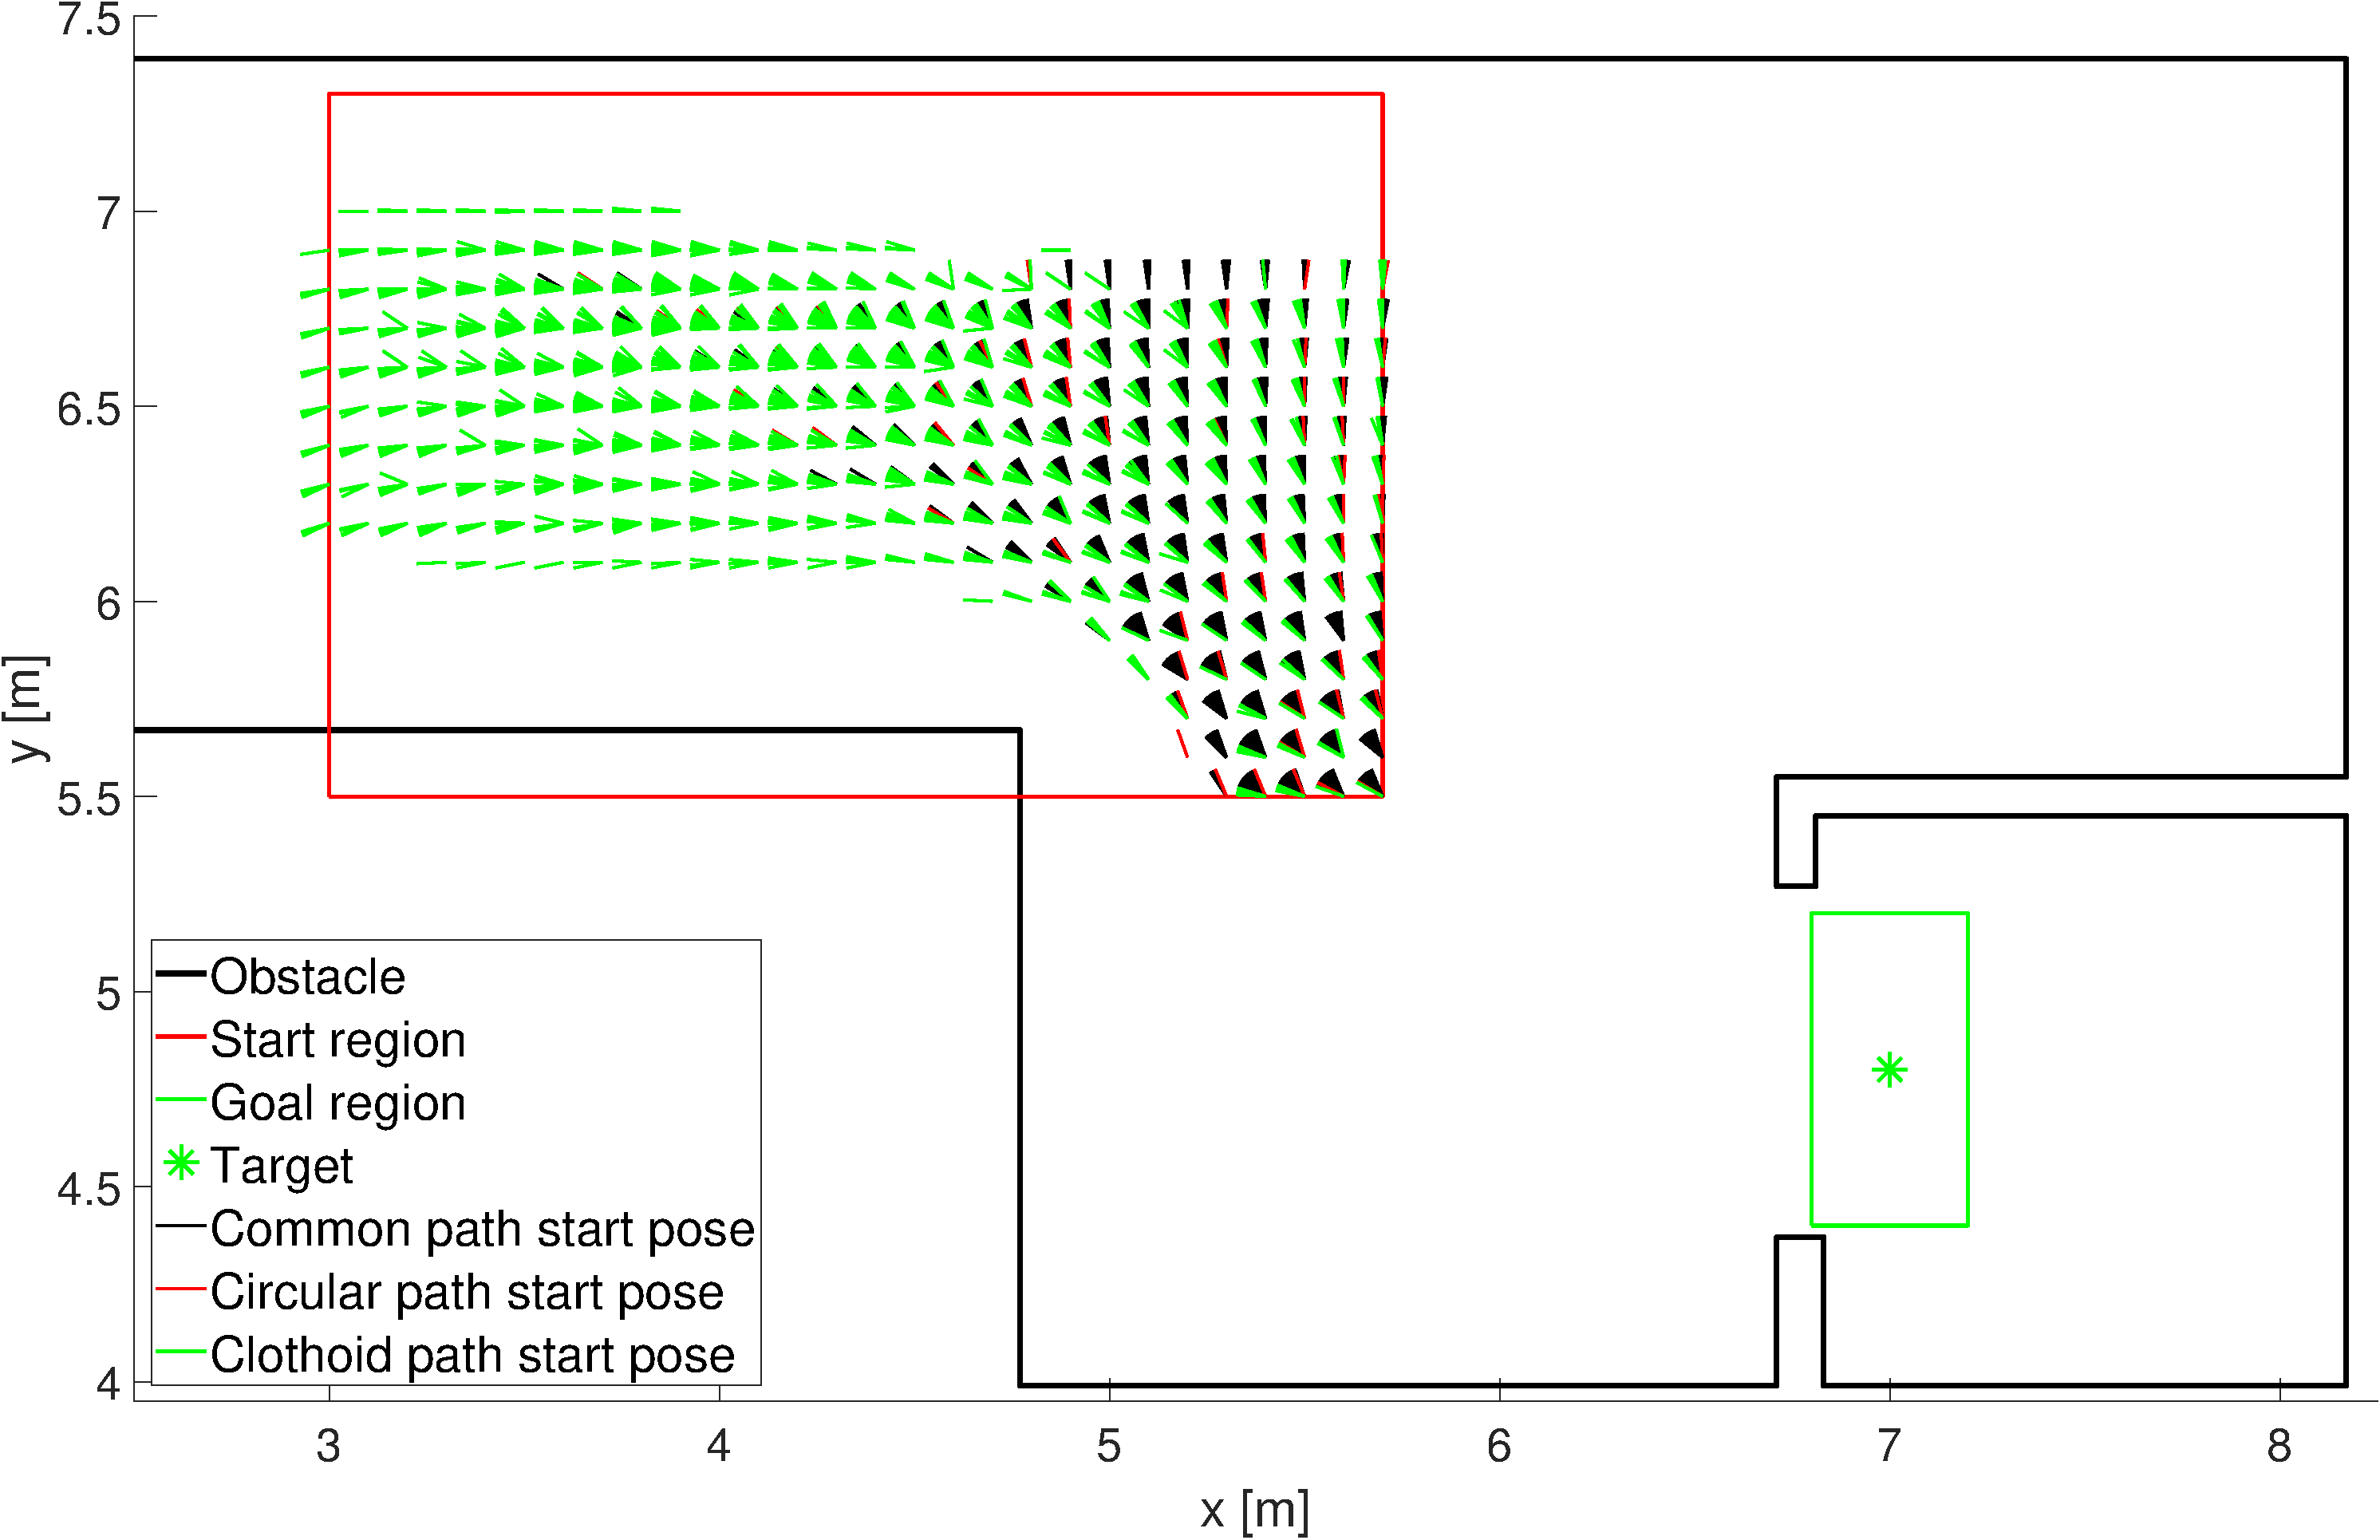
\includegraphics[width=\textwidth]{EnterLiftEval_result.pdf}
     \doublecaption{Successful start poses for each LPT planning a path backwards into an elevator}{separated in the three different cases\label{fig:EnterLiftEval_result}}
\end{figure}

\begin{figure}[!htbp]
	\centering
    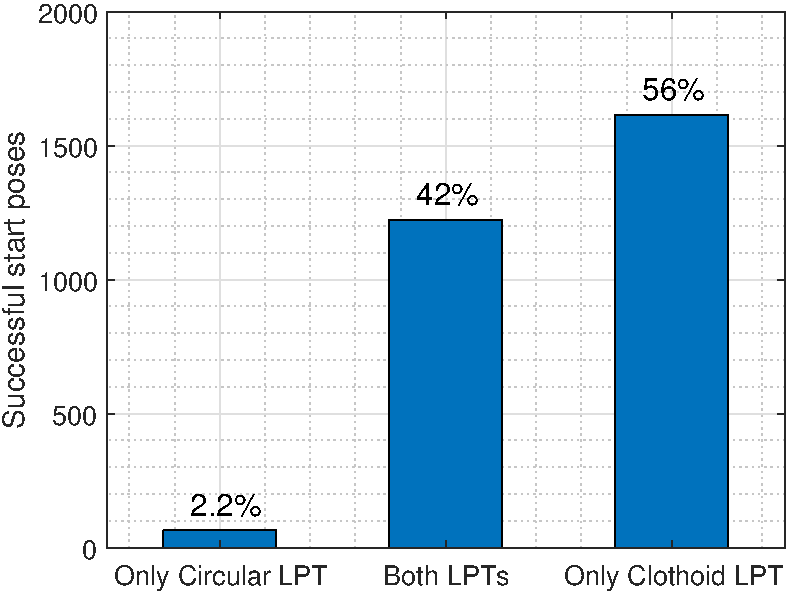
\includegraphics[width=0.5\textwidth]{EnterLiftEva_hist.pdf}
     \doublecaption{Histogram illustrating the outcome of the different cases for planning a path backwards into an elevator.}{There are in total 2904 successful start poses, from which 1224 are common to both LPTs. Whereas 64 are only from the circular LPT and 1616 from the clothoidal LPT. \label{fig:EnterLiftEva_hist}}
\end{figure}

\newpage

\section{Time Performances} \label{sec:EvalTP}
One important consequence of augmenting the number of paths in the set of feasible trajectories of the LPTs is the time needed to adjust the path length. Since the clothoidal LPT has six times more paths than the circular LPT and assuming a stable computing capacity, applying the clothoidal LPT would be impracticable if the increase in time required would be fully proportional to the increased number of paths. 

This section will investigate two different cases. First, in \cref{sec:EvalTimeSingle} a single occupied cell of the lookup table presented in \cref{sec:OBLT} will be simulated as occupied. Then, in a more realistic scenario, the sAMR is positioned in several poses in the environment as shown in \cref{fig:EnterLiftEval_result}, resulting in a different amount of occupied cells from the lookup table \cref{sec:EvalTimeMulti}.

The presented benchmarks were run on a computer with an Intel\textregistered~Core\texttrademark~i5-4460 quad core 3.20GHz CPU with 16GB of memory. Benchmark scripts were written in MATLAB. A better time performance is therefore expected when this developed LPPA would be implemented in a more efficient programming language (e.g. C/C++), as the results available for the circular LPT \cite{DemeesterEtAl2012}. The relative comparison between the two LPTs remains however relevant.

\subsection{Single Occupied Cell} \label{sec:EvalTimeSingle}
This benchmark will show the time needed to adapt the path length of both LPTs when a single cell of the LPT is simulated to be occupied. This has been visually demonstrated in \cref{fig:LPT_LT}. To avoid any bias with respect to the row-index in the lookup table, an equally spread set of occupied cells will be picked from the whole lookup table. The algorithm used for this search is the build-in MATLAB function ``ismember'' which was applied on a hash-table form of the lookup table to further optimize speed. This hash-table form enables a scalar-search compared to a much slower row-search. This speed-up optimization was found in \cite{Altman2014} and has approximately accelerated the search time by a factor of 50.

\Cref{fig:TimeBench_SingleObs_mat} (left) shows a histogram of the obtained execution time of this benchmark applied to the circular and clothoidal LPT. The circular LPT proves to be more time efficient, which was expected, since this LPT contains six times less paths compared to the clothoidal LPT. The median execution time of the circular LPT is 0.265 ms compared to 0.608 ms for the clothoidal LPT (2.3 times slower). 


Another important relationship that can be analyzed with this benchmark is the execution time dependency of the affected paths (for 1 occupied cell). This is shown in \cref{fig:TimeBench_SingleObs_mat} (right), where each dot indicates a single experience. From this figure, a clear dependency on the number of paths can be seen, with the linearly increasing minimal execution time, for a cell affecting a particular amount of paths. This reflects the linear increasing time needed to adapt the length of each individual path. The vertical difference in time can be explained by a varying time needed for searching the cell in the lookup table.

%TODO  read this again
As expected, the maximum number of paths from the circular LPT (250) is to be found on the plot in red. This is not the case for the clothoidal LPT composed of 1500, however the cell containing the maximum amount of paths is 337. Since not every path from the clothoidal LPT starts at the origin due to the EP (recall \cref{sec:EP}, some trajectories are composed of 2 clothoids). There is a parent-child from clothoids originating from a certain EP, since they are automatically marked as fully blocked from the moment the path leading to that EP has been shortened. This structural relationship has therefore led to an increase in the speed for the collision checking, since otherwise the graph displayed in \cref{fig:TimeBench_SingleObs_mat} (right) would have continued linearly to 1500 paths affected by a single cell. 

\begin{figure}[!htbp]
	\centering
	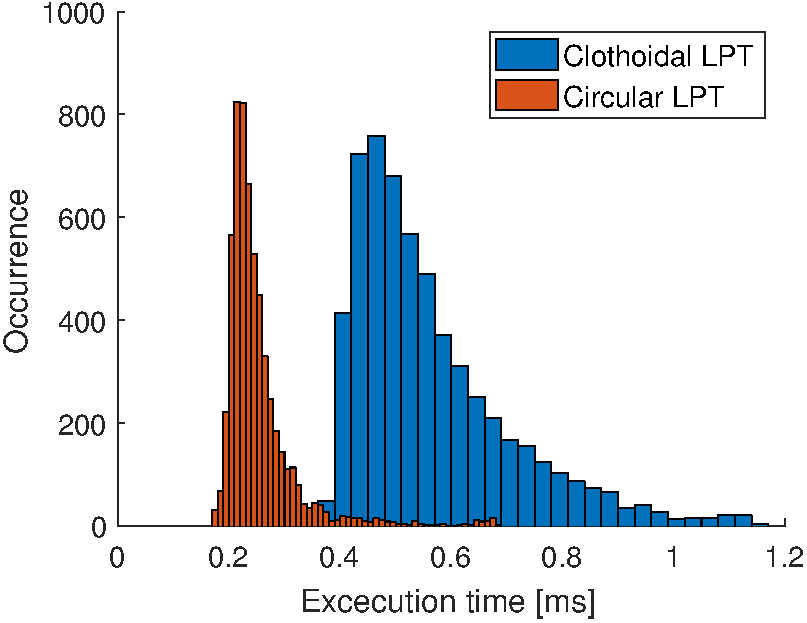
\includegraphics[width=0.45\textwidth]{TimeBench_SingleObs_mat_hist.pdf}
    \hfill
	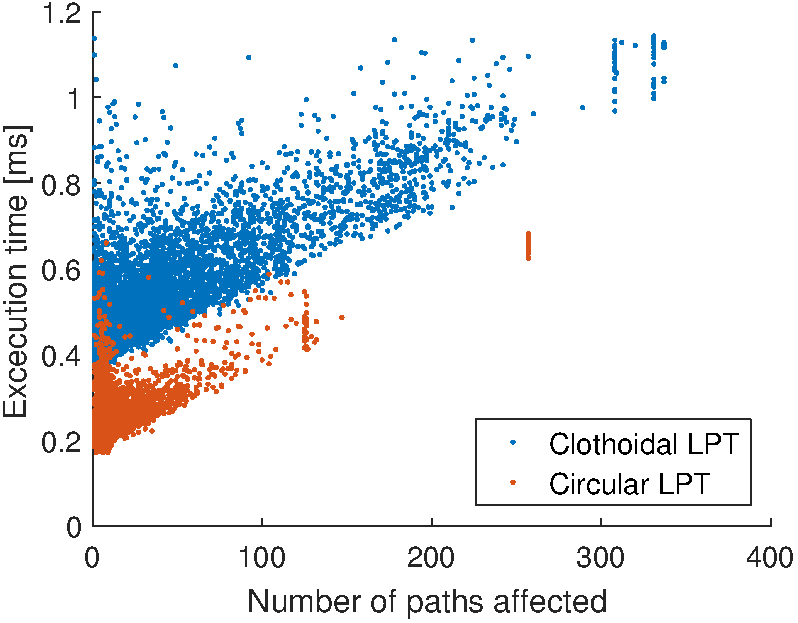
\includegraphics[width=0.45\textwidth]{TimeBench_SingleObs_mat_PathInfluence.pdf}
    \doublecaption{Execution time needed to adapt the path length of the circular and clothoidal LPT for a single obstacle.}{Occupied cells are equally spread over the whole lookup table to obtain cells affecting a different number of paths. (left) Histogram of the resulting execution time. The circular LPT with a median of 0.265 ms is 2.3 times faster as the clothoidal LPT with a median of 0.608 ms. (right) When plotting the executing time over the number of paths the cell affects, a clear linear relationship is visible for the minimal executing time for both LPTs, reflecting the linear increasing time needed to adapt each path. The varying amount of execution time for a given number of paths per cell can be explained by the difference in time needed to find that cell in the lookup table.\label{fig:TimeBench_SingleObs_mat}}
\end{figure}

\subsection{Multiple Occupied Cells} \label{sec:EvalTimeMulti}
This benchmark will evaluate the execution time of both LPTs in a simulated environment (\cref{fig:EnterLiftEval_result}). Different start poses are tested resulting in a varying amount of occupied cells from the environment matched with cells in the lookup table. \Cref{fig:TimeBench_MultiObs} (left) shows a histogram of the execution time needed to adapt each path from the LPTs. The relative difference in execution time is more visible in this case compared to a single occupied cell. For this benchmark, the median execution time of the circular LPT is 29 ms compared to 114 ms for the clothoidal LPT; the clothoidal LPT is therefore 3.9 times slower.

\Cref{fig:TimeBench_MultiObs} (right) shows the execution time of the trajectory adjustment over the number of occupied cells. No clear relationship can be observed, which indicates that the process of matching occupied grid cells from the environment with the precomputed cells in each LPT is the most expensive operation. One can note the slightly more grouped nature (already visible from the histogram) of the circular LPT compared to the clothoidal LPT.

\begin{figure}[!htbp]
	\centering
	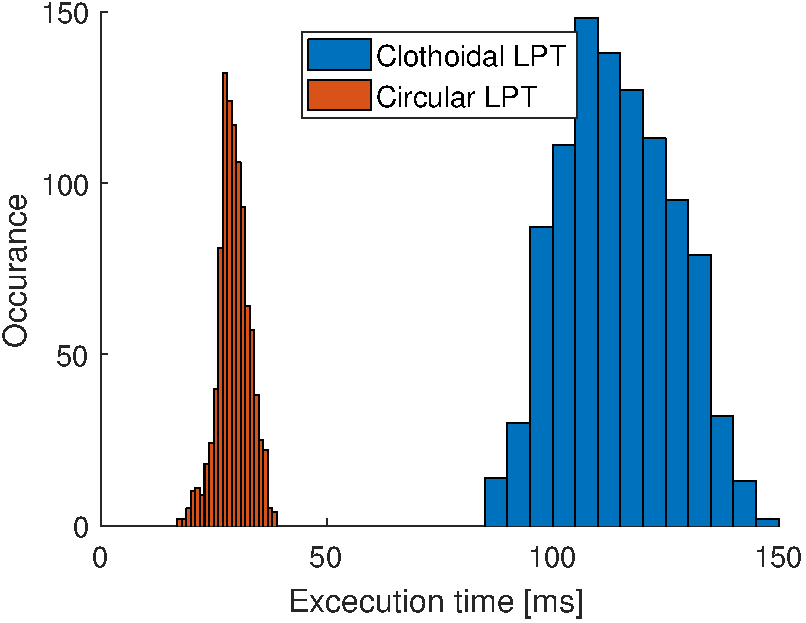
\includegraphics[width=0.45\textwidth]{TimeBench_MultiObs_hist.pdf}
    \hfill
	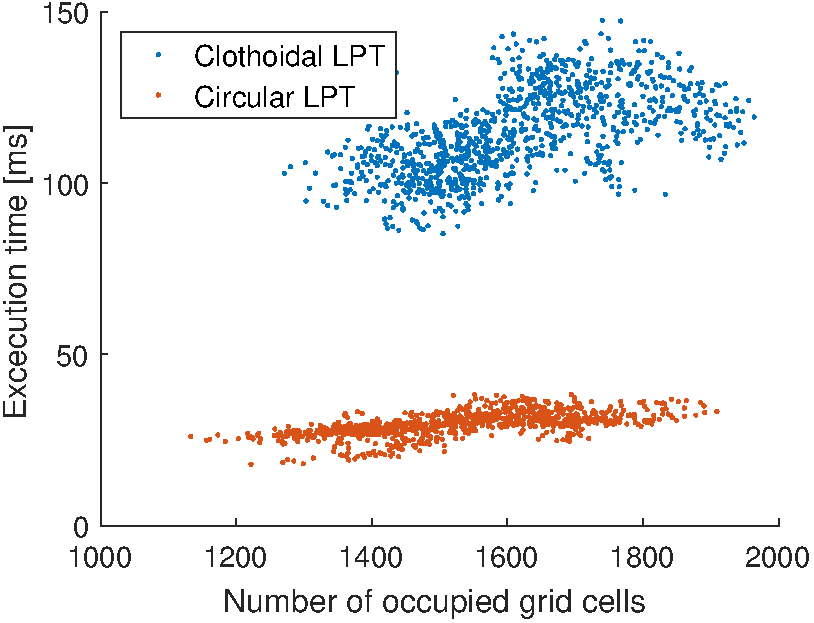
\includegraphics[width=0.45\textwidth]{TimeBench_MultiObs_ObstacleInfluence.pdf}
    \doublecaption{Execution time needed to adapt the path length of the circular and clothoidal LPT for a simulated environment.}{Different poses are used to obtain a varying number of triggered cells when an obstacle in the surroundings of the sAMR matches one in the precomputed lookup table. (left) Histogram of the resulting execution time. The circular LPT with a median of 29 ms is 3.9 times faster as the clothoidal LPT with a median of 114 ms. (right) When plotting the executing time over the number of occupied cells from the lookup table, no clear relationship can be found. This indicates that the search function is the most time-consuming process.\label{fig:TimeBench_MultiObs}}
\end{figure}
\newpage

\section{Conclusion} \label{sec:EvalConc}
This chapter has evaluated two critical performance criteria of the developed local path planner designed in \cref{cha:Design}, the clothoidal LPT by comparing it to the circular LPT. The clothoidal LPT has a less restrictive formulation compared to the circular LPT, therefore enabling more complex curves. 

By having six times more paths compared to its predecessor, the clothoidal LPT achieves an improved path planning performance. This has been demonstrated in two different situations. The clothoidal is especially successful in situations that either require a complex path to achieve a possible destination due to the environment as per the first experiment, or that have an unfavorable start pose, as per the second experiment.

 A major concern is the extra time needed to adapt the paths from the clothoidal as against those of the circular LPT. The time performance of each LPT has been evaluated, in an experience whereby both LPTs were tested in an environment with varying test poses. This resulted in varying the number of occupied grid cells from the environment matching the cells from the lookup table. Results of this experience showed that the clothoidal LPT needed nearly four times more computing time to adjust each individual path length as compared to the circular LPT (median value of 114 ms compared to the 29 ms). 
 
 Although these experiments have been performed in MATLAB and implementing this in a more efficient programming language (e.g. C/C++) would minimize the impact of the increased computing time, it may be important to achieve further efficiency improvements. The main reason behind the large amount of paths for the clothoidal LPT is due to the use of EPs as explained in \cref{sec:EP}. These are uniformly spread over the local grid, resulting in a symmetric expansion of the paths of the LPT (recall \cref{fig:LSLClothoid}). Two possible improvements regarding the position of the EPs could be implemented:
\begin{enumerate}
\item An asymmetric location of the EPs is applied, yielding for example 6 different zones (straight, left, right for forwards or backwards motion). Six different LPT are then available for the LPP then only has to choose between the six possible LPTs, for instance straight-forward or left-backwards.
\item The choice of the EP positions is performed online and is not necessarily restricted to 2 successive clothoids.  The fast calculations of the LPT could therefore be combined with the flexibility of DMP by using a fast planner for several successive EPs. 
\end{enumerate}
Both solutions would achieve a more efficient clothoidal LPT, by taking the environment or the previous user’s intention into account, without interfering with the improved planning capacity resulting from the higher flexibility of the clothoid.
